\documentclass[a4paper, 12pt]{report}
\usepackage[english]{babel}
\usepackage[utf8]{inputenc}
\usepackage[T1]{fontenc}
\usepackage{lmodern}
\usepackage[Conny]{fncychap}
\usepackage{enumerate}
\usepackage{listings}
\usepackage{color}
\usepackage{import}
\usepackage{listings}
\usepackage{caption}
\usepackage{url}
\usepackage[backend=bibtex]{biblatex}
\usepackage{amsmath}
\usepackage{graphicx}
\usepackage{tikz}
\usetikzlibrary{calc, shadings, shadows, shapes.arrows, chains}

% Numbers and units
\usepackage[squaren, Gray]{SIunits}
\usepackage{sistyle}
\usepackage[autolanguage]{numprint}
\usepackage{fullpage}
\usepackage{hyperref}
\usepackage{multirow}
\usepackage{xparse}
\usepackage{enumitem}
\usepackage{amsmath}

\bibliography{./biblio}

\setlength{\parskip}{1em}

\definecolor{codegreen}{rgb}{0,0.6,0}
\definecolor{codegray}{rgb}{0.5,0.5,0.5}
\definecolor{codepurple}{rgb}{0.58,0,0.82}
\definecolor{backcolour}{rgb}{0.95,0.95,0.92}

\lstdefinestyle{mystyle}{
backgroundcolor=\color{backcolour},
commentstyle=\color{codegreen},
keywordstyle=\color{magenta},
numberstyle=\tiny\color{codegray},
stringstyle=\color{codepurple},
basicstyle=\footnotesize,
breakatwhitespace=false,
breaklines=true,
captionpos=b,
keepspaces=true,
numbers=left,
numbersep=5pt,
showspaces=false,
showstringspaces=false,
showtabs=false,
tabsize=2
}

% Styles for interfaces and edge labels
\tikzset{%
interface/.style={draw, rectangle,font=\tiny},
ethernet/.style={interface, fill=yellow!50},% ethernet interface
speed/.style={anchor=south, font=\tiny},% line speed at edge
route/.style={draw, shape=single arrow, single arrow head extend=2mm,
minimum height=1cm, width=2cm, white, fill=blue!20,
drop shadow={opacity=.8, fill=blue!50!black}, font=\tiny}% inroute / outroute arrows
}

\lstset{style=mystyle}

\newcommand*{\captionsource}[2]{%
  \caption[{#1}]{%
    #1%
    \\ \textbf{Source:} #2%
  }%
}

\newcommand*{\shift}{1.3cm}% For placing the arrows later

\newcommand\si[2]{\numprint[#2]{#1}}
\newcommand\np[1]{\numprint{#1}}

\newcommand\figref[1]{figure~\ref{fig:#1}}

\NewDocumentEnvironment{myfig}{mm}
{\begin{figure}[!ht]\centering}
{\caption{#2}\label{#1}\end{figure}}

%%%% SPACING %%%%
\renewcommand{\baselinestretch}{1.3}
\headsep = 10.mm
%%%% CHOOSE MARGINS %%%%
\usepackage{geometry}
\geometry{hmargin=2.5cm,top=3cm,bottom=2.3cm}
%%%% COMMANDS %%%%
%%%%%%%%%%%%%%%%%%%%%%%%%%%%%%%%%%%%% CHANGE HERE %%%%
\renewcommand\title{Multipath TCP and OpenVPN}
\newcommand\name{Alois Paulus \textsc{}}
\newcommand\options{}
\newcommand\supervisor{ \textsc{}}
\newcommand\readerone{ \textsc{}}
\newcommand\readertwo{ \textsc{}}
\newcommand\years{20..-20..}
%%%% BEGIN %%%%

\begin{document}

  \nocite{*}

  %%%% COVER %%%%
  \thispagestyle{empty}
  \noindent\begin{minipage}{.25\textwidth}
  \noindent
\includegraphics[width=3.6cm]{./images/ucl.jpg}
  \end{minipage}
  \begin{minipage}{.5\textwidth}
  \begin{center}
  UNIVERSITE CATHOLIQUE DE LOUVAIN
  \\~\\~
  ECOLE POLYTECHNIQUE DE LOUVAIN
  \\~\\~\\~\\~\\~
  \end{center}
  \end{minipage}
  \begin{minipage}{.25\textwidth}
  \hfill
\includegraphics[width=3.6cm]{./images/epl.jpg}
  \\~\\~\\~\\~
  \end{minipage}
  \vspace{4.5cm}
  \begin{center}
  \bfseries{\scshape{\Huge{\title}}}
  \end{center}
  \vspace{4.5cm}
  \begin{minipage}{.5\textwidth}
  \begin{tabular}{ll}
  Supervisor: Olivier Bonaventure & \supervisor
  \\ Readers: Gregory Detal & \readerone
  \\          Marc Lobelle & \readertwo
  \end{tabular}
  \\~\\~
  \end{minipage}
  \begin{minipage}{.5\textwidth}
  \begin{tabular}{l}
  Thesis submitted for the Master's degree
  \\ in computer science and engineering
  \\ options: SINF2M1
  \\ by Alois Paulus
  \end{tabular}
  \end{minipage}
  \vfill
  \begin{center}
  Louvain-la-Neuve
  \\ Academic year 2014-2015
  \end{center}
  %%%% END COVER %%%%

  \newpage

  \tableofcontents

  \newpage


 \chapter{Introduction}
  \section{Introduction}

  Having a fast and reliable internet connection is something that individuals and compagnies would want.

  Nowadays, there are multiple solutions to this, for example compagnies can get a fiber optic connection but it is still very expensive.

  Individual or small entreprise have Multihoming. It uses multiple internet connections at the same time and balances traffic amongst them using a router configured especially for that.
  Unfortunatly it does not always improve the speed of the connection and can be slow to react to failures.

  In this paper, I describe and analyse another solution which is less expensive than optic fiber and will make better use of brandwidth
  and be more tolerant to failures than Multihoming. This solution implies using MultiPath TCP, OpenVPN and OpenWRT.

  Multipath TCP (MPTCP) has been implemented by the IP Networking Lab at Université catholique de Louvain(UCL) in Louvain-la-Neuve for the linux kernel. It is an extension of the TCP protocol,
  and it's goal is to support the use of multiple transport paths between a pair of hosts.
  The benefits of MPTCP include a performance improvement in term of throughput and a better handling of failures.

  OpenVPN is an open source application implementing a virtual private network (VPN) to create secure connections between hosts over a network.
  OpenWrt is a linux distribution for embedded devices typically home routers. It is built from the ground up to be a full-featured, easily modifiable and light weight operating system.

  In this setup, MPTCP will be use to balance the traffic between multiple internet connections and recover from a possible failure of one of them.
  OpenVPN will be use to create the link between the MPTCP compatible server and the home router running a modified version of OpenWRT supporting MPTCP.
  For this to work, the user/entreprise should have two or more internet connections and a server with a high brandwith running a MPTCP kernel.

  The goal of the solution described in this paper is to give the possibility to more people to get a fast and reliable internet connection.

  This paper will first present the theory about multipath TCP and Virtual Private Network in Chapter 1. Chapter 2 describes the setup of the experiment and the tests operated.
  The results of these tests are presented in Chapter 3. Chapter 4 is an attempt to develop solutions to the problems encountered duriing the test. Finally, Chapter 5 presents the tools used
  to perform the tests and Chapter 6 concludes the report.

  \section{Multipath TCP (MPTCP)} \label{sec:mptcp_exp}

  Multipath TCP has been implemented by the IP Networking Lab at Université catholique de Louvain(UCL) in Louvain-la-Neuve for the linux kernel.
  MPTCP is an attempt to solve problems of the TCP protocol : the inability to move TCP connection from one IP to another and the inability to use more than one path for a single TCP connection.
  Many attempts have been made but some involve changes in the applications and others lose advantages of current TCP protocol.

  Multipath TCP also need to be backward compatible with normal TCP to ensure that even if the other end is not compatible they can still communicate.
  Another thing to achieve is the fairness between MPTCP and TCP: if MPTCP and normal TCP share a bottleneck link, MPTCP should not be able to use more bandwith than a normal TCP connection.

  \subsection{Architecture}

  Multipath TCP is an extention of the TCP protocol,. It does not change the interface of the socket API for applications which allows all applications to benefit from it
  without need for modification.
  It removes the strong link between IP and TCP so that devices can use multiple IP for a single MPTCP connection.

  MPTC uses TCP options to annonce MPTCP support and communicate MPTCP informations between host.

  The setup of a MPTCP connection is as follow:

  \begin{enumerate}
    \item First the initiator of the connection annonces that he is MPTCP compatible (MP\_CAPABLE)
    \item Then if the receiver is MPTCP compatible, it establish a new MPTCP connection
    \item After that, it adds new subflow on every know path to the existing MPTCP connection (MP\_JOIN)
    \item Finally it transmit data on the MPTCP connection
  \end{enumerate}

  \begin{figure}[h!]
    \centering
    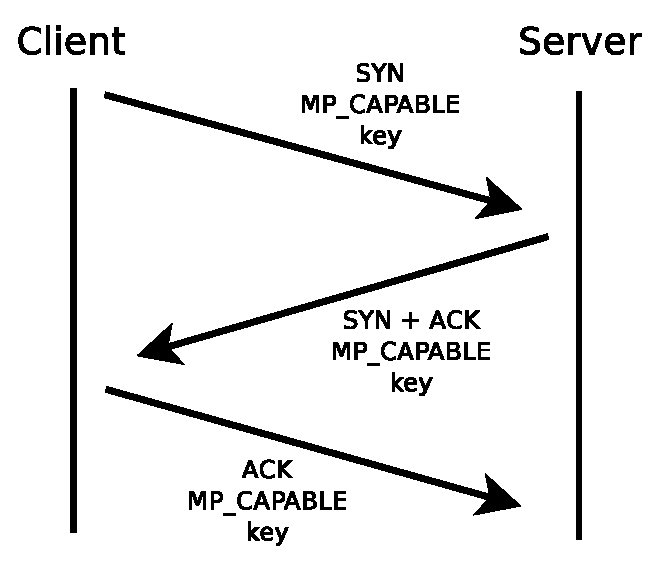
\includegraphics[width=8cm]{./images/mptcp_connection_setup.eps}
    \caption{MPTCP connection setup}
    \label{mptcp_connection_setup}
  \end{figure}


  To establish a MPTCP connection it uses a three-way handshake as show in figure \ref{mptcp_connection_setup}.
  A client send a packet having the MP\_CAPABLE option to tell the server he is compatible.
  The server send back a ACK containing a MP\_CAPABLE option and a random key if it is compatible.
  After that the client send a ACK to the server containing the key, this will setup the first subflow.

  \begin{figure}[h!]
    \centering
    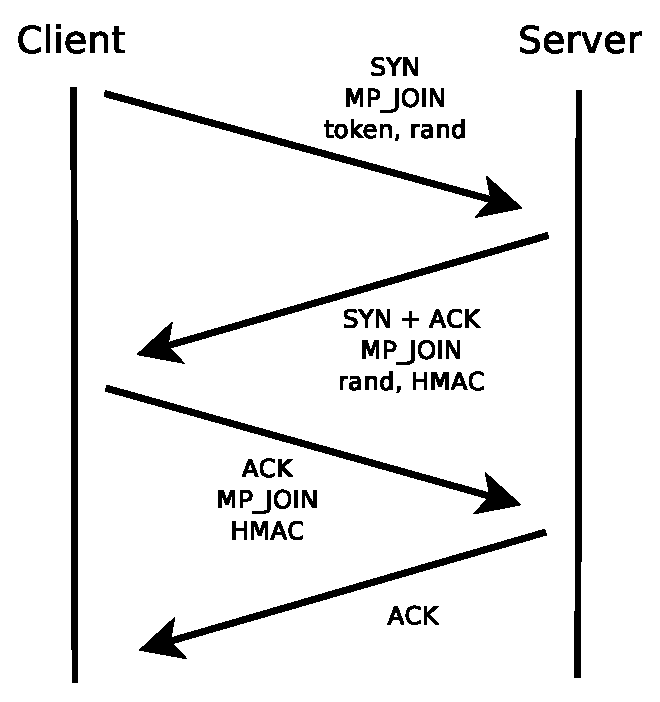
\includegraphics[width=8cm]{./images/mptcp_mp_join.eps}
    \caption{MPTCP Add subflow}
    \label{mptcp_mp_join}
  \end{figure}

  If the client has more than one physical link connected with the server, MPTCP will try to add another subflow to the existing connection.
  For this it will use a three-way handshake and the MP\_JOIN option with a unique token.(figure \ref{mptcp_mp_join})

  \begin{enumerate}
    \item First a SYN with the MP\_JOIN Option, a unique token and random key will be sent
    \item Then the client and the server will compute an hash-based message authentification code computed over the random key exchanged.
  \end{enumerate}

  The token is there to be able to uniquely identify a subflow, because in normal TCP a connection is identified by <srcip,srcport,dstip,dstport>
  which in this case is not sufficient to uniquely identify a subflow in case of a host behind a NAT.

  When multiple subflows have been established, data can be transmited over any of them. This can be used to increase the throughput of the connection or
  to retransmit data if one subflow fail. Each subflow is equivalent to a single TCP connection.

  If multiple subflows are use for a single TCP connection MPTCP must decide on which one to send the data and how much data.
  For this purpose, MPTCP use a scheduler, there are two type of scheduler in MPTCP :

  \begin {enumerate}
    \item The default scheduler used by MPTCP will first send data on subflows with the lowest RTT until their congestion-window is full then it will start transmitting on the subflows with the next higher RTT.
    \item The roundrobin scheduler will transmit X consecutive segment on each path in a round robin fashion (X can be changed and default is 1).
  \end{enumerate}

  Using multiple subflows also require to order the data within each subflow and then order the data between these different subflows, because some can be faster than others.
  When receiving data it first reorders them at the subflow level using the subflow sequence number, a 32bits number. Then it reorders the data between the different sublows at the connection level using the data sequence number.

  \subsection{Congestion}

  Congestion control in MPTCP is more complex than with regular TCP because it uses multiples subflows for one connection.
  On these subflows the level of congestion can be very different, if one uses standard TCP congestion algorithm the performance for MPTCP it usually become unfair to regular TCP and
  in some situations decreases the performances.

  To solve that problem a few congestion control algorithms have been developped for MPTCP like LIA, OLIA, wVegas. These algorithms are described below.

  \subsubsection{ Linked Increase Algorithm (LIA)} \label{sec:lia}

  The LIA algorithm has three main goals :

  \begin{enumerate}
    \item Having a total throughput bigger than the one TCP can get using the best path
    \item Not being more aggressive than TCP, be fair to TCP.
    \item Balancing the congestion over paths
  \end{enumerate}

  As it accomplishes the two first goal but fails to accomplish the third one,  a new algorithm has been developped, OLIA.

  In LIA, the slow start, fast retransmit, and fast recovery algorithms, as well as the multiplicative decrease of the congestion avoidance state are the same as in standard TCP.

  What changes is the increase phase of the congestion avoidance state, the window is increased by the minimum between the increase that would get normal TCP and the computed increase
  for the multipath subflow. The computed increase is calculated using a parameter $\alpha$ which defines the aggresiveness of the MPTCP flow. The value of this parameter $\alpha$ is chosen such that the aggregate
  throughput of the multipath flow is equal to the rate a TCP flow would get if it ran on the best path.
  $\alpha$ need to be calculated for each MPTCP flow. The formula which is used has been derived by equalizing the rate of the multipath flow with the rate of a TCP running on the best path.

  This guarantees the goal number two: not being more aggressive than TCP. Goal one is accomplished by computing an increase for the multipath subflow equal to
  the throughput a TCP flow would get if it ran on the best path.

  \subsubsection{ Opportunistic Linked-Increases Algorithm (OLIA)} \label{sec:olia}

  OLIA is a window-based congestion-control algorithm that couples the increase of congestion windows and uses unmodifed TCP behavior in the case of a loss.
  Like LIA, the algorithm only modifies to the increase part of the congestion avoidance phase.

  It uses a set of best paths devided in two, a set with max windows and the rest of the paths. For the paths that have a small windows, OLIA increase the window faster.
  For the path that have the max windows, the increase is slower.

  \subsubsection{ wVegas } \label{sec:wvegas}

  wVegas is a delay-based congestion control based on TCP vegas. It is more sensitive to change because it does not have to wait for packet losses to react and shift between subflows to adapt to network congestion.
  For each subflow it calculate the difference between the expected sending rate and actual sending rate

  During slow-start it double the congestion window every other RTT. If the difference is bigger than a threshold, it switches to congestion-avoidance.
  During congestion-avoidance it increase the window by one packet every RTT if the difference is small otherwise it reduces it by one packet.

  This means that overall the window grow slower than other algorithm and this avoids losses. However when the BDP is large, it switches too fast to the congestion avoiding phase and gives
  bad throughput because the windows is too small.

  \subsection{Usages}

  MPTCP can be use in different fields. It is usefull for devices like smartphones that have multiple network interfaces with different throughput and latency. Today these devices only use one interface at a time and
  if it loses the connection to that interface, all the currently open TCP connection will be terminated and will need to be reopenned.

  This is a situation that MPTCP can solve by having one subflow for the 3G interface and one subflow over the wifi interface: when one subflow fails, the data are sent over the other subflow.

  MPTCP can also be very usefull in data center where different topologies use multiple paths accross the server layer and the traffic need to be balanced between the paths to avoid congestion.

  \section{VPN}

  A Virtual private network provide a point-to-point connection between two or more nodes on top of an existing network, it create a tunnel between the connected nodes.(figure \ref{vpn1})

  In VPN privacy is a concern: The data which are transmited using these virtual network need to be encrypted so that if someone intercept it on the global network, it cannot be read.
  The data are encrypted before entering the tunnel and will be decrypted after leaving it, the VPN will usually add extra header information to the packets for the remote node to be able to decrypt.

  Another technique used in VPN is the authentification. Client and server must provide information about who they are so that they can prove their idendity.
  This is mostly done by using a Message Authentication Code (MAC).

  One of the main motivation for VPN is that it is cheaper to use multiple virtual networks implemented on a global network than use multiple smaller physical networks.
  It is usually used by compagnies to create a private network over the internet.

  There are several types of VPN technologies : Point-to-Point Tunneling Protocol,Secure Socket Layer/Transport Layer Security (SSL/TLS) or Internet Protocol Security.
  They all use the same basic principle to transfert data accross by tunneling it.

  \begin{figure}[h!]
    \centering
    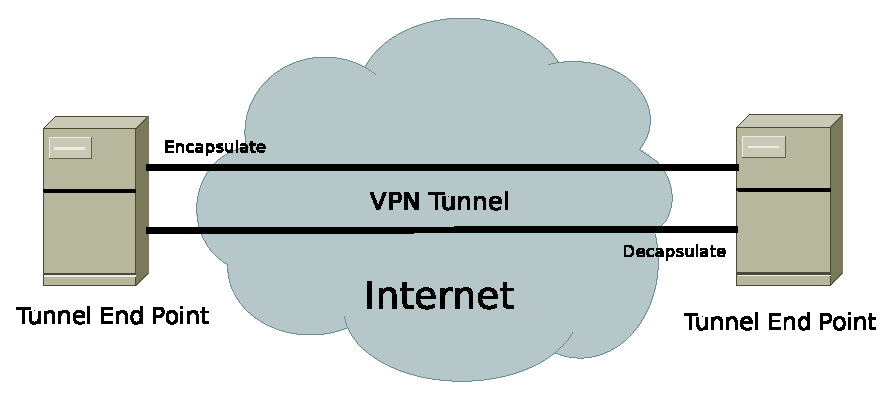
\includegraphics[width=1\textwidth]{./images/vpn1.eps}
    \caption{VPN Tunnel}
    \label{vpn1}
  \end{figure}

  The principle is that the packet is encrypted and encapsulated within another packet which will be delivered to the other node. The node will then decapsulate the packet and decrypt it.

  \subsection{Why using a VPN}

  For this article, we will use a end-to-end, one-to-one connection to connect the router and the server with each other and encapsulate all the clients traffic into the OpenVPN tunnel.

  So even in the case clients do not support MPTCP, all the packets sent by the client will be encapsulated on the router within OpenVPN packet
  and because the router is MPTPC capable, the OpenVPN packets will use MPTCP to transit between the router and the server.

  \subsection{OpenVPN} \label{sec:section_openvpn}

  OpenVPN is an open source application implementing a virtual private network to create secure connections over a network, it is developped by James Yonan.

  It uses SSL/TLS in its custom security protocol and uses the OpenSSL library to do the encryption of data and the authentication.
  There are several authentication methods like static key, certificate or username/password.
  Using Encryption is more secure but needs more ressource because packets need to be decrypted.

  OpenVPN uses two channels, a data channel that carries the users' IP datagrams and a control channel that handles key negotiation and configuration.

  OpenVPN can use UDP or TCP to transport the packets and provide several security feature. UDP is usually advised because it is generaly faster.

  OpenVPN is available on a lot of operating system : Linux, Windows, Mac OS X and multiples router firmware such as DD-WRT, OpenWRT ...
  This gives the possibility to make your router act as a OpenVPN client and users connected to that router can access a VPN without having to install OpenVPN on their computers.

  \begin{figure}[h!]
    \centering
    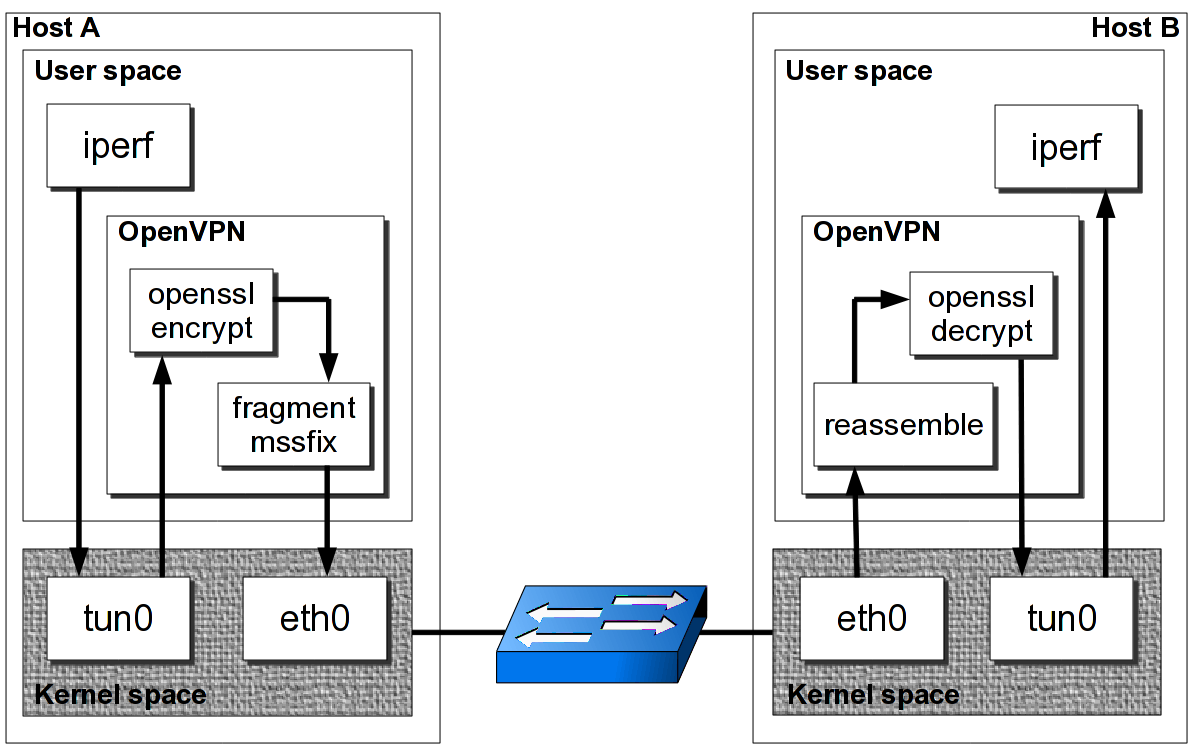
\includegraphics[width=1\textwidth]{./images/packetflow.png}
    \caption{VPN Packets flow}
    \label{packetFlow}
  \end{figure}

  OpenVPN runs in user space which provides good security and portability but packets need to travel between kernel space and user space which is called context switching.
  Context-switching takes CPU cycle, which can impact a lot the performances if the hardware is not powerfull enough.

  On figure \ref{packetFlow} you can see how the packets flow from an application to the network and from the network to the application.

  To create the tunnel OpenVPN uses the tunnel driver that is provided as a module for linux. This driver enable the creation of virtual interfaces called tun or tap devices. The difference between tun and tap are the
  layer at which they are, tap is a layer 2 and tun is a layer 3 device.

  In practice this means that tap is able to send ethernet frame and add more overhead and tun is only able to send packet but add less overhead. For the tests presented in this paper the interface tun is enough and is a better
  choice because it add less overhead.


 \chapter{Setup}
  \section{Setup}


  \begin{figure}[h!]
    \centering
    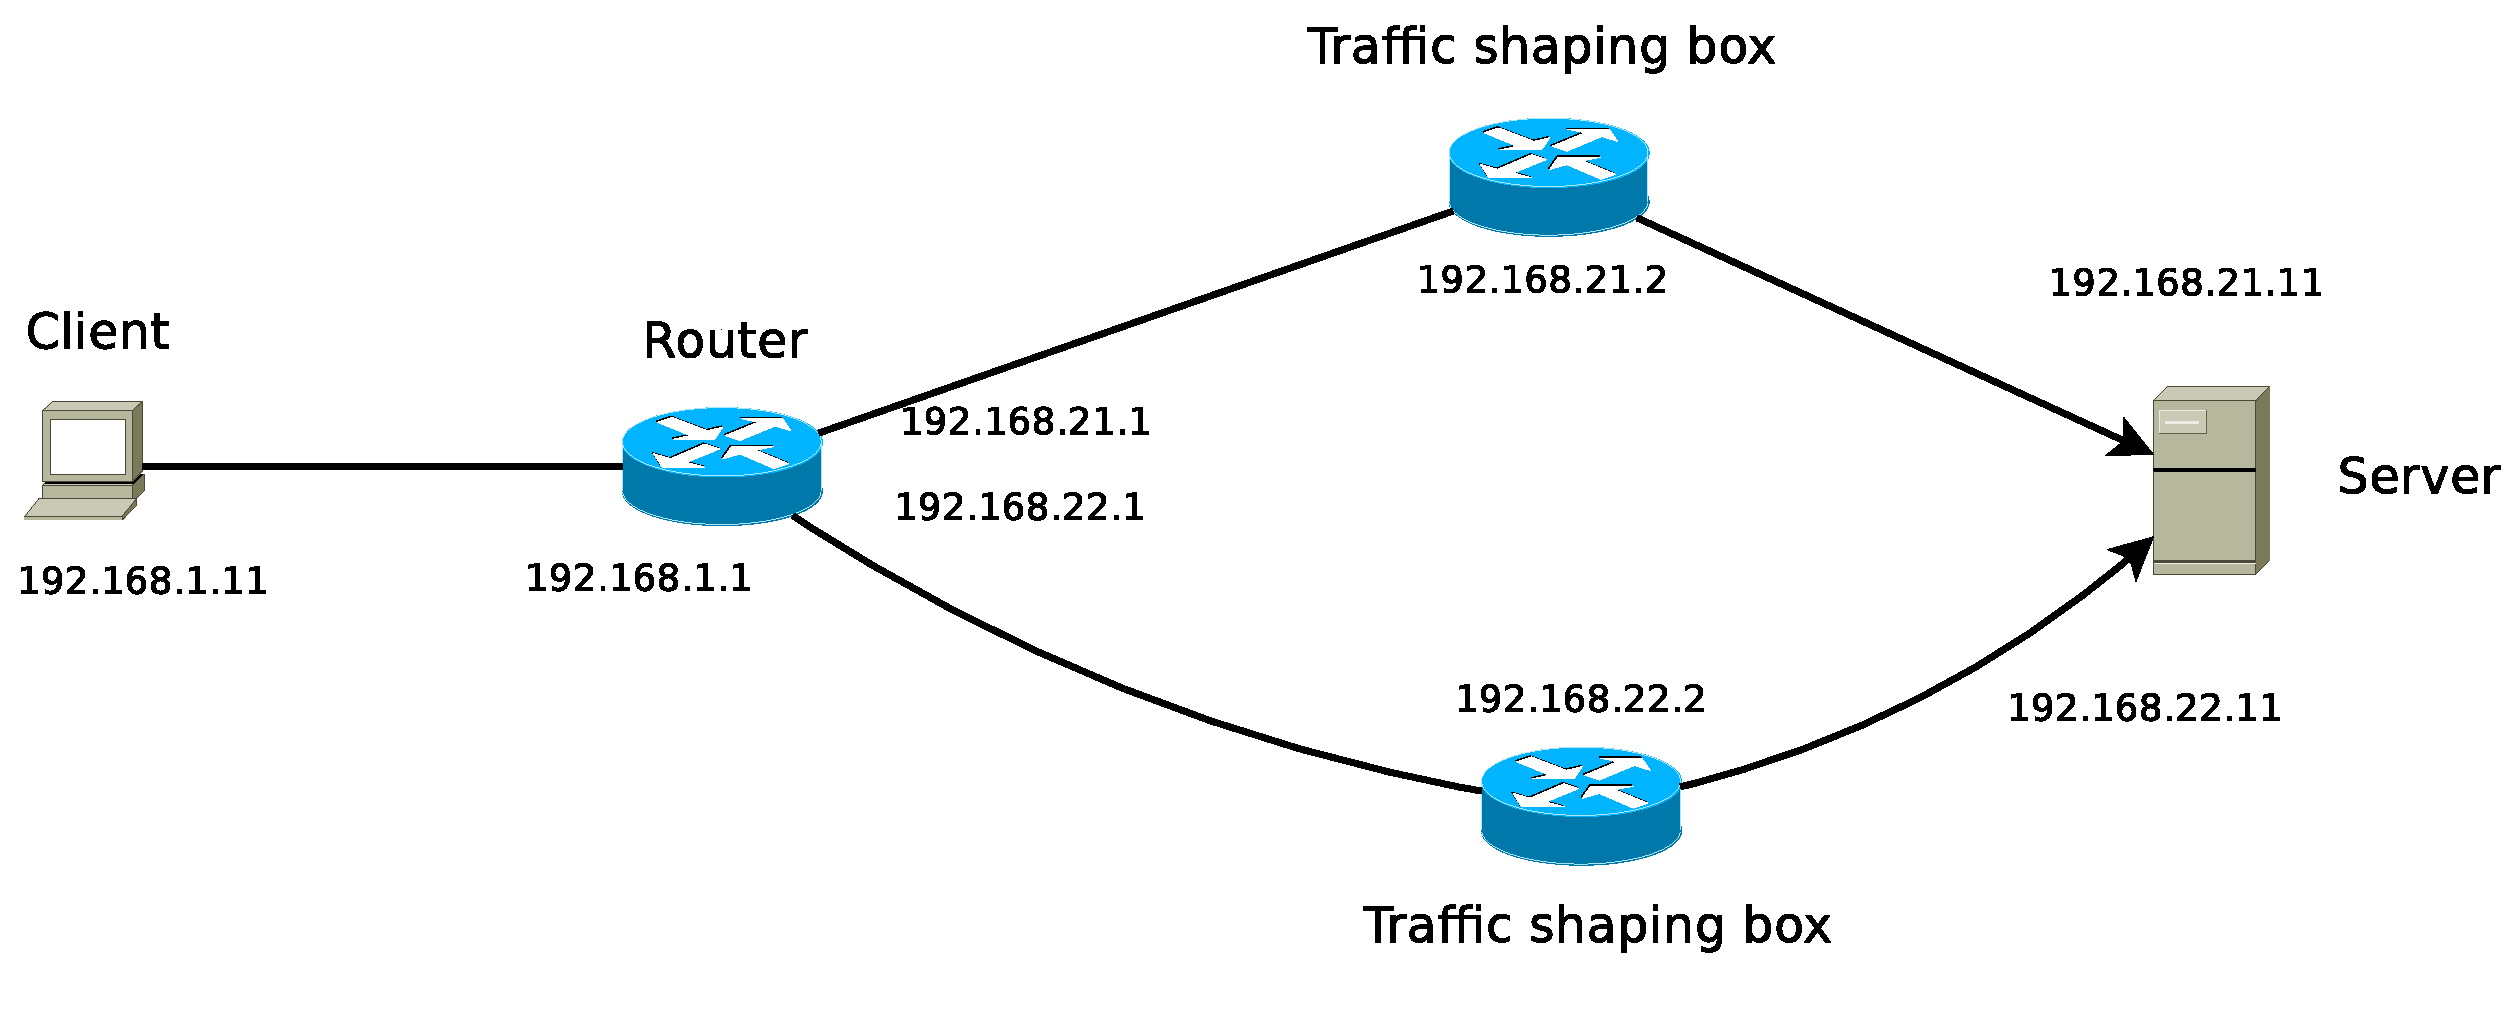
\includegraphics[width=12cm]{./images/setup.eps}
    \caption{Setup}
    \label{setup_fig}
  \end{figure}

  As show in figure ~\ref{setup_fig} the setup consists of five machines :

  \begin{itemize}
    \item One home computer, a client.
    \item One server for the OpenVPN server
    \item One home router connected to the OpenVPN server, by two ethernet cable to enable MPTCP to use two subflows.
    \item Two routers to do some traffic shaping.
  \end{itemize}

  \subsubsection{OpenVPN client}

  It is a TP-LINK N900 router, its CPU is a PPC P1014@800MHz and it has 128Mb of RAM \autocite{openwrt_n900}.
  It will be running OpenWRT with a custom kernel 3.10.49 with MPTCP v0.89.0-rc compiled by Sébastien Barré and Gregory Detal.

  \subsubsection{Traffic shaping boxes}
  The traffic shaping boxes will mainly limit the brandwith and add delay between the router and the server to emulate real internet connections speed.
  They are TP-Link TL-WR741ND router, CPU Atheros AR7240 @ 350 MHz and 32Mb of RAM. It will be running OpenWRT with tc, a shaping software, installed.

  \subsubsection{OpenVPN server}
  The OpenVPN server is a computer with a Intel Pentium 4 CPU and 2Go of RAM.
  It will be using debian running kernel 3.14.33 from the MPTCP Github repository \ref{mptcp} with MPTCP v0.89.5 compiled with all the TCP congestion algorithms.

  The client computer will connect to the router and access the server through it.

  For the purpose of these tests we decided not to use encryption or authentification on the OpenVPN tunnel, mainly because it need more CPU power and the TP-LINK N900 is not powerfull.
  Using encryption and authentification would have decrease performances and given that the main goal of this paper is not security, encryption is not needed.

  \subsection{OpenVPN configuration} \label{sec:openvpn_config}

  Listing~\ref{lst:openvpn_config_client} presents the important parameters in the OpenVPN configuration file. The whole configuration can be found in the annexes.

  \begin{lstlisting}[caption={Openvpn configuration},label={lst:openvpn_config_client}]
  auth none
  cipher none
  sndbuf 0
  rcvbuf 0\end{lstlisting}

  As \textit{auth} and \textit{cipher} are about encryption and anthentification, they are disable because, as explained earlier,
  they add more overhead to packet and are not needed for these tests because privacy is not our concern.

  \textit{sndbuf} and \textit{rcvbuf} are two very important settings that are used by OpenVPN to set the \textit{SO\_SNDBUF} and \textit{SO\_RCVBUF} options on individual socket with setsockopt.
  The \textit{SO\_SNDBUF} and \textit{SO\_RCVBUF} options are the send and receive buffer size.
  When they are set to 0, OpenVPN does not set value with setsockopt and the value from the OS are used.

  After reading quite a lot about these two parameters the most common advise for Linux is to use a value of 0 for \textit{sndbuf} and \textit{rcvbuf} because it let the
  OS taking care of adjusting the TCP window size.

  For the purpose of the tests in this paper, it is important to keep control on the size of the TCP window to be able to evaluate their impact.
  Consequently, I will set values for \textit{sndbuf} and \textit{rcvbuf} manually.

  The advantage of using these settings instead of set globally the value with the help of sysctl is that it only affect sockets created by OpenVPN and not all
  the sockets and it is easier to change.

  \subsection{Delay boxes}

  The two delay boxes are placed between the OpenWRT router and the server, one for each link. Their goal is to limit the bandwidth and introduce delay on links.

  For this I used tc, a traffic control tool in the linux kernel, used to configure and control the network schedulers. It enables to choose between a sets
  of queing systems and mechanisms to control how the packets are received and transmitted. This is usually called QoS (Quality of service).

  It gives the possibility to :
  \begin{itemize}
    \item Limit the total bandwidth of a link using TBF or HTB
    \item Give priority to latency sensitive traffic
    \item Distribute unreserved bandwidth equitably
    \item Reserve bandwidth for a particular application
    \item Limit the bandwidth of a particular user, service or client
    \item Introduce delay, loss, duplication, reordering (netem)
  \end{itemize}

  From the many possibilities offered by tc, I use in this paper the first and the last one, using TBF and netem.
  Here is an example :

  \begin{lstlisting}
    # tc qdisc add dev eth0 root handle 1:0 tbf rate 8mbit burst 50k latency 5ms
    # tc qdisc add dev eth0 parent 1:1 handle 10: netem delay 50ms
  \end{lstlisting}

  The first line of this script will add a \textit{qdisc} which is a scheduler to the interface \textit{eth0}. The handle is the name given for this \textit{qdisc} on the interface \textit{eth0}.
  The handle is defined by a number of form major\:minor, it is followed by a class type, tbf which is a queuing discipline to attach to the \textit{qdisc}.
  It will limit the rate to 8mbit and set the buffer to 50k.

  The second line add a class to the interface \textit{eth0} on the parent handle (from line 1). Again we give a handle and then we give the class type,
  netem. It will add a delay of 50ms to the interface \textit{eth0}.

  In this example we use netem to add delay to the link and then use TBF to add a bandwidth limit. This simple process is adequate to our needs.


    \begin{figure}[h!]
     \centering
     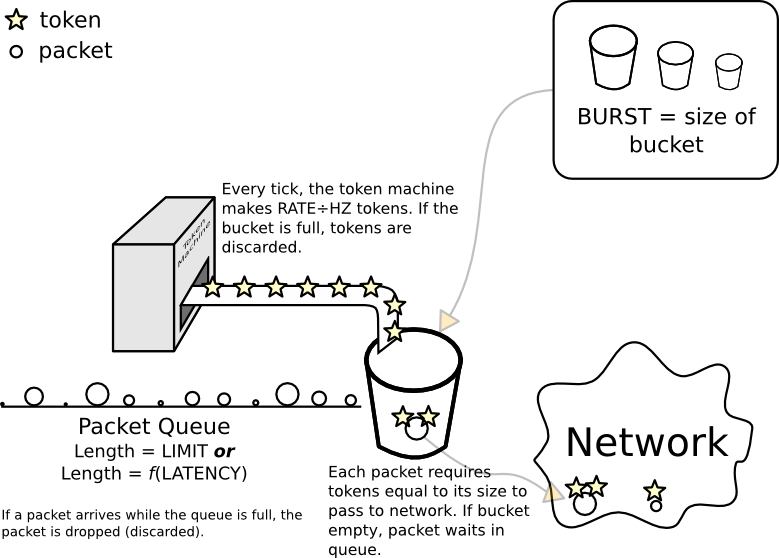
\includegraphics[width=8cm]{./images/tc.png}
     \captionsource{Token Bucket Filter}{\cite{stackoverflowtbf}}
     \label{fig_tbf}
    \end{figure}

    Figure \ref{fig_tbf} presents how TBF works in practice. The burst parameter is equivalent to the size of the bucket, it holds a limited amount of tokens and if
    too many are added the bucket overflows and the tokens are lost.

    The latency or limit is the number of packets that can sit into the line waiting to get a token.
    This occurs when the bucket is empty or if the bucket does not have enough tokens for all the packets.

    When the kernel send a packet it first needs to obtain a tokens.
    If it does not obtains a token it is put in a line to wait for a token and if this line is full it is dropped.

  \section{Tests Procedures}

  To mesure the differences in term of performance when using OpenVPN we will measure the throughput, the delay and the CPU usage using different configurations such as follow :

  \begin{enumerate}
    \item UDP protocol as OpenVPN protocol
    \item TCP protocol as OpenVPN protocol with MPTCP using 2 links (2 subflow)
  \end{enumerate}

  The tests will be ran using different link speed to mimic real internet connection speed.
  For that I looked for the different FAI in Belgium and listed their available speeds in April 2015.

  Here are the one selected for the tests :
  \begin{itemize}
    \item  8mbps (edpnet)
    \item  32mpbs (voo telenet)
    \item  100mbps (numericable)
  \end{itemize}

  Delay will also be introduces on the links to see how the performances may vary.
  \begin{itemize}
    \item  1ms
    \item  25ms
    \item  200ms
  \end{itemize}

  \subsection{Bulk data transfer}

  A common type of network traffic on the internet especially with the cloud is bulk data transfers.
  It is used when pulling files from a FTP or accessing data on your shared drive (google drive or dropbox).

  To simulate this type of traffic, I use the TCP\_MAERTS a test from Netperf, it measure bulk data transfer performance. This will measure how fast the server can send data to the client.

  \subsubsection{TCP\_MAERTS}

  TCP\_MAERTS test open a single TCP connection to the remote machine and makes as many rapid write calls as possible. These write calls have a specific size which by default is the sender buffer send size.

  The socket buffers on either end will be sized according to the systems default and all TCP options will be at their default settings.

  Options :
  \begin{itemize}
\item -s size Sets the local socket send and receive buffers (size in bytes)
\item -S size Sets the remote socket send and receive buffers (size in bytes)
\item -m size Sets the local send message size to size
\item -M size Sets the remote receive message size to size
\item -D Sets the TCP\_NODELAY socket option on both the local and
remote systems
  \end{itemize}

  \subsection{TCP Request/Response}  \label{sec:setup_request_response}

  Another common type of network traffic on the internet between client and server is the request/response model.
  This model is based on individual transactions between the client and the server.
  The client sends a request to the server, the server receives it, process it and sends a response back to the client.

  To mimic this type of traffic, the TCP\_CRR test from Netperf will be used.
  Apache Benchmark (AB) will also be used because the  TCP\_CRR is sequential and it is interesting to analyse the impact on the results when multiple connections are used at the same time.
  The server will have a Apache server with the default settings and will serve the default apache welcome page.

  \subsubsection{TCP\_CRR}

  TCP\_CRR measures the performances of establishing a connection, exchanging a single request/response transaction, and tearing-down that connection.
  This is similar to the process of an HTTP 1.0 or HTTP 1.1 connection when HTTP Keepalives are not used. It is a synchronous, one transaction at a time, request/response test.
  By default the message size is 1 byte but it can be changed using options.

  Options :
  \begin{itemize}
\item -r req,resp sets the size of the request or response message, or both
\item -s size sets the size of the local socket send and receive buffers to
size bytes
\item -S size sets the size of the remote socket send and receive buffers to
size bytes
\item -D sets the TCP\_NODELAY socket option on both the local and
remote system
  \end{itemize}

    \subsubsection{Apache Benchmark (AB)}
    Apache Benchmark (AB) is a tool for benchmarking HTTP server. It shows how many request per second the server can deliver to the client by sending a arbitrary number of concurrent request.
    It has been created to benchmark the Apache web server.

    \section{Git Repository}

    To make all the tests reproductable, I have try to automize as much as possible, using mainly python and bash script.
    Everything is avaible on a git repository on Github \url{https://github.com/alokhan/memoire}.

    In this repository you find all the configuration files used for the router and server, all the script used to generate the graphics,
    ,all the \textit{.csv} files containing the test results used for this paper and also some documentation.


 \chapter{Tests results}
   This section prensent the test results.

  Firstly I  present the performance difference between TCP and UDP used as the OpenVPN protocol by testing the throughput and the number of request/response per second.
  Secondly I test the behavior of MPTCP using link with different RTT and bandwith.
  Finally I try different congestion control and analyse wether it help increasing performances.

 \section{TCP vs UDP}

  In this section I compare the througput of a TCP connection using TCP and UDP as the OpenVPN tunnel protocol to determine where MPTCP can be interesting and where not.
  Many combinaison of bandwidth and delay will be used they will be specified for each test.
  The size of the openvpn buffers will also be specify as it plays a role in the overall throughput.
  TCP windows autotuning mechanism of Linux will always be enable.

  \subsection{Bulk data transfer} \label{sec:bulk_data_transfer}

  This first test is a bulk data transfer.

  Test setup :

  \begin{itemize}
  \item First link bandwith of 8mbit/s, 32mbit/s, 100mbit/s  and RTT: 2ms (default route)
  \item Second link bandwith of 8mbit/s, 32mbit/s, 100mbit/s  and RTT: 2ms
  \item Using default mptcp scheduler
  \item OpenVPN buffer default size 65536 bytes on client and server
  \item Congestion control : cubic
  \end{itemize}

  \begin{figure}[h!]
    \centering
    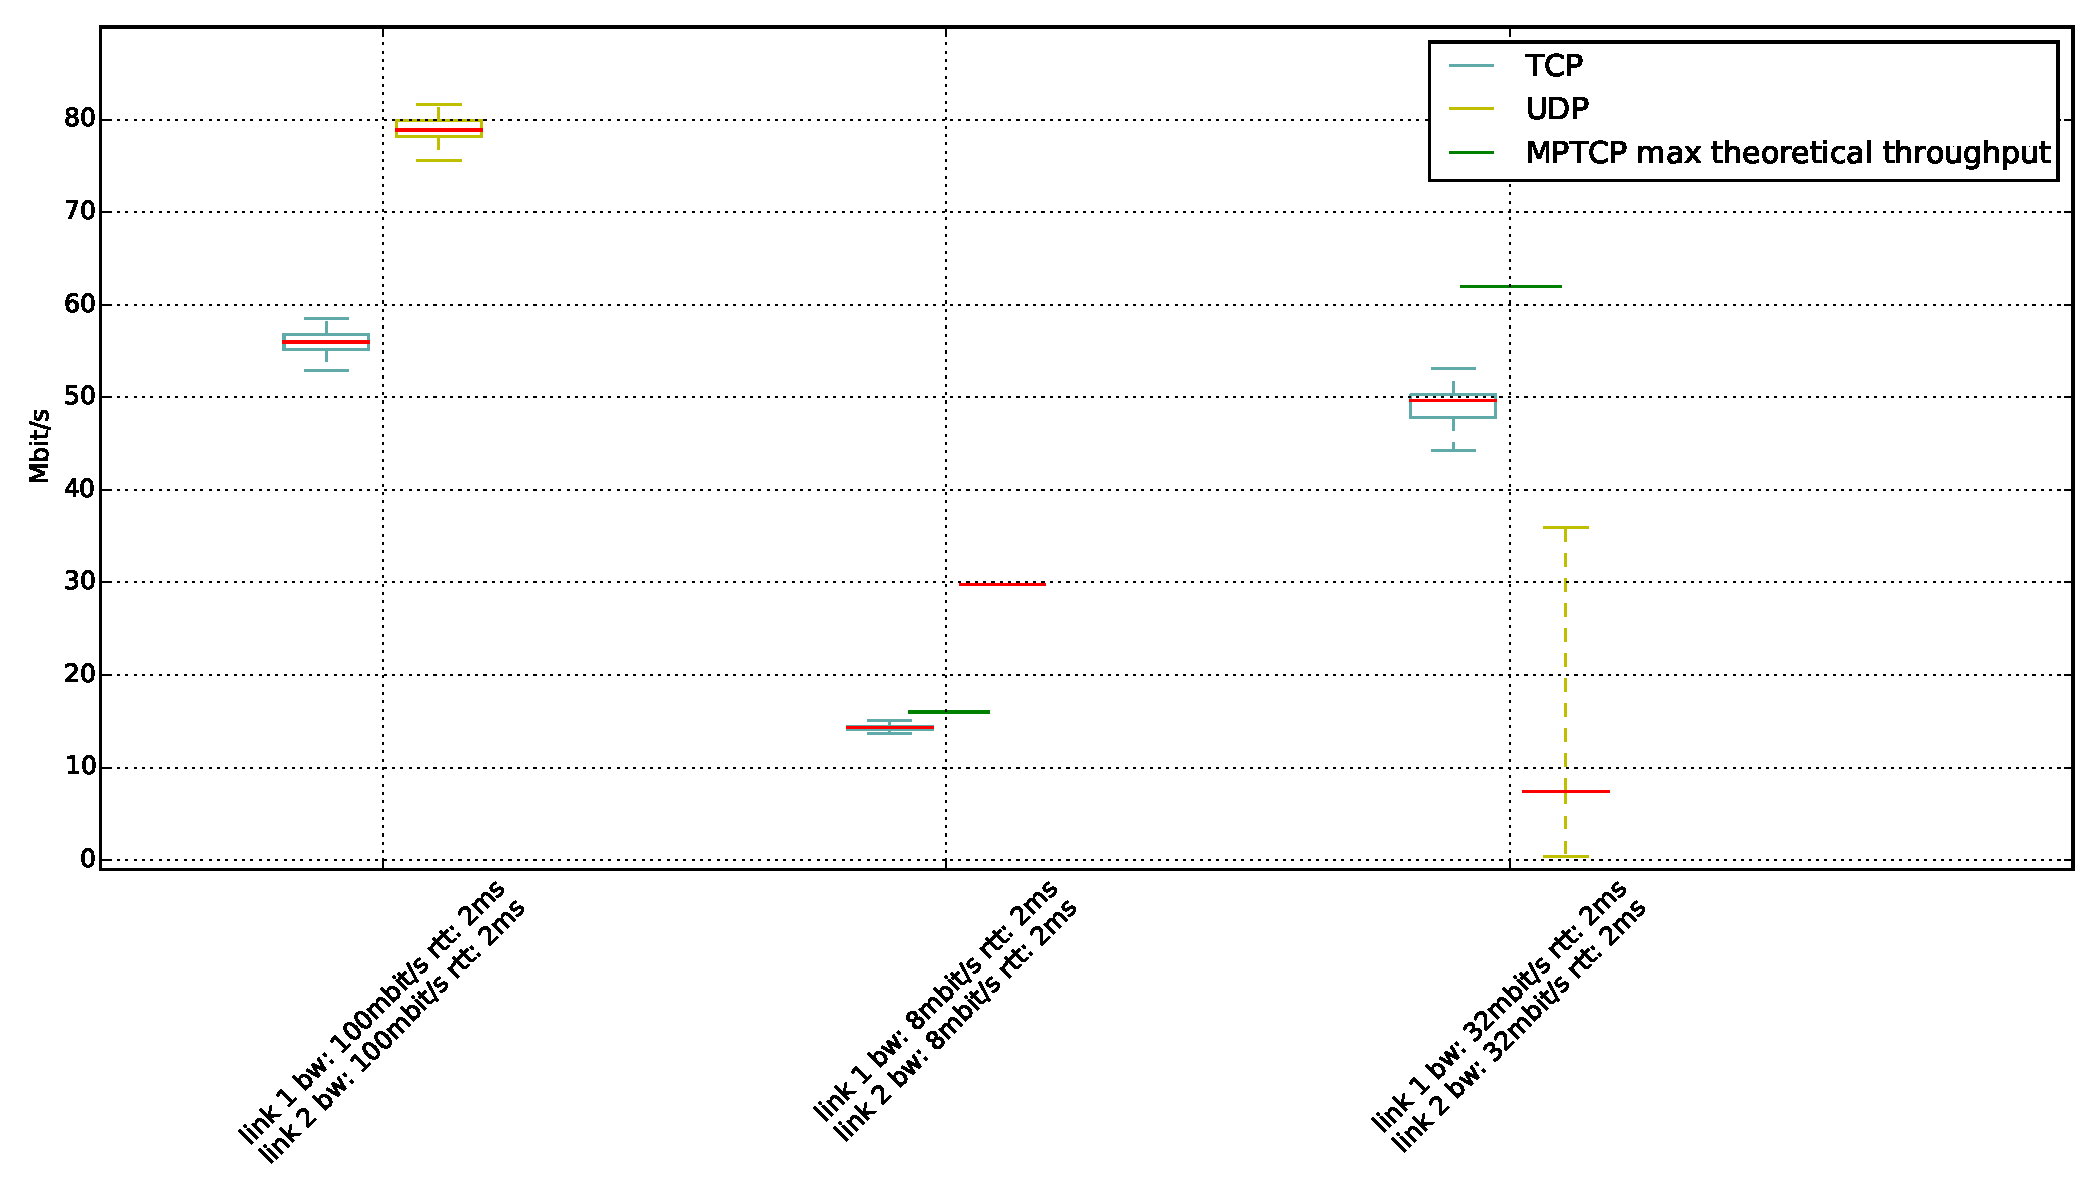
\includegraphics[width=14cm]{../results/tcp_vs_udp_2ms.pdf}
    \caption{TCP vs UDP RTT: 2ms Buffer size: 64k}
    \label{all_tcp_vs_udp}
  \end{figure}

  When using TCP as the OpenVPN protocol, MPTCP will creates two subflows, one on each link. Actually the full-mesh path manager create four subflow on this setup
  but the cross IP subflows has been blocked with the help of IPTables rules. On the other hand UDP will only use one of the available links.

  For this test my hypothesis is that using MPTCP would always give a better throughput because it can use double of the bandwith than UDP can.

  However results in figure \ref{all_tcp_vs_udp} shows that TCP is faster than UDP for small maximum bandwidth like 8 or 32mbit/s but for greater maximum bandwidth like 100mbit/s,
  TCP is slower than UDP.

  Besides, for the 32mbit/s bandwidth, the capacity of the two links are not fully used otherwise the throughput would be of about 60-64mbit/s.
  Further, even when using UDP and a maximum of 100mbit/s bandwidth, the whole bandwidth available is not used.

  These results are mainly due to two things :
  \begin{enumerate}
    \item The router CPU is used at about 100\% while the tests are running for the 32mbit/s (tcp) and 100mbit/s (tcp and udp) maximum link bandwidth
    \item TCP over TCP can be bad because it can trigger multiple retransmissions \cite{tcpovertcp}
  \end{enumerate}

The first reason is linked to the fact that the router has to encapsulate and decapsulate the packet from the OpenVPN tunnel as explained in section \ref{sec:section_openvpn}
causing the router to switch between kernel space and
userspace. This is very costly in CPU cycle and the router CPU is a bit too weak.

The second reason relates to having two layers of TCP connection.
TCP is a protocol that assumes an unreliable carrier. So if you have multiple layers of TCP connections each layer will guarantee that every data arrive to the other end.
If the encapsulating or Internet layer drops a packet, both TCP streams will attempt to correct the error and retransmit duplicate data.
This queues up data transmissions exponentially and slow down the data transmission.

Bofre concluding, it is interesting to analyse how the traffic was split accross the subflows. For this, I used \textit{tcpdump} to capture packets and \textit{mptcptrace} to analyse these captures.
The traffic was captured on the OpenVPN server, on the sending side, to avoid having too much stress put on the router.

The sequence graphic generated by mptcptrace showed that the traffic was well splitted accross the subflows, which is the expected result because the scheduler used during these tests was the default and both links had the same RTT and same bandwidth.

Figure \ref{mptcptrace_subflow} showshow the traffic was split. When the green line approaches the $+1$ limit,
it is the initial subflow which is mainly use and when the blue line approaches the $-1$ limit it is the second subflow which is mainly use.
Here, the two lines are near 0, meaning that they are both used equaly.

  \begin{figure}[h!]
    \centering
    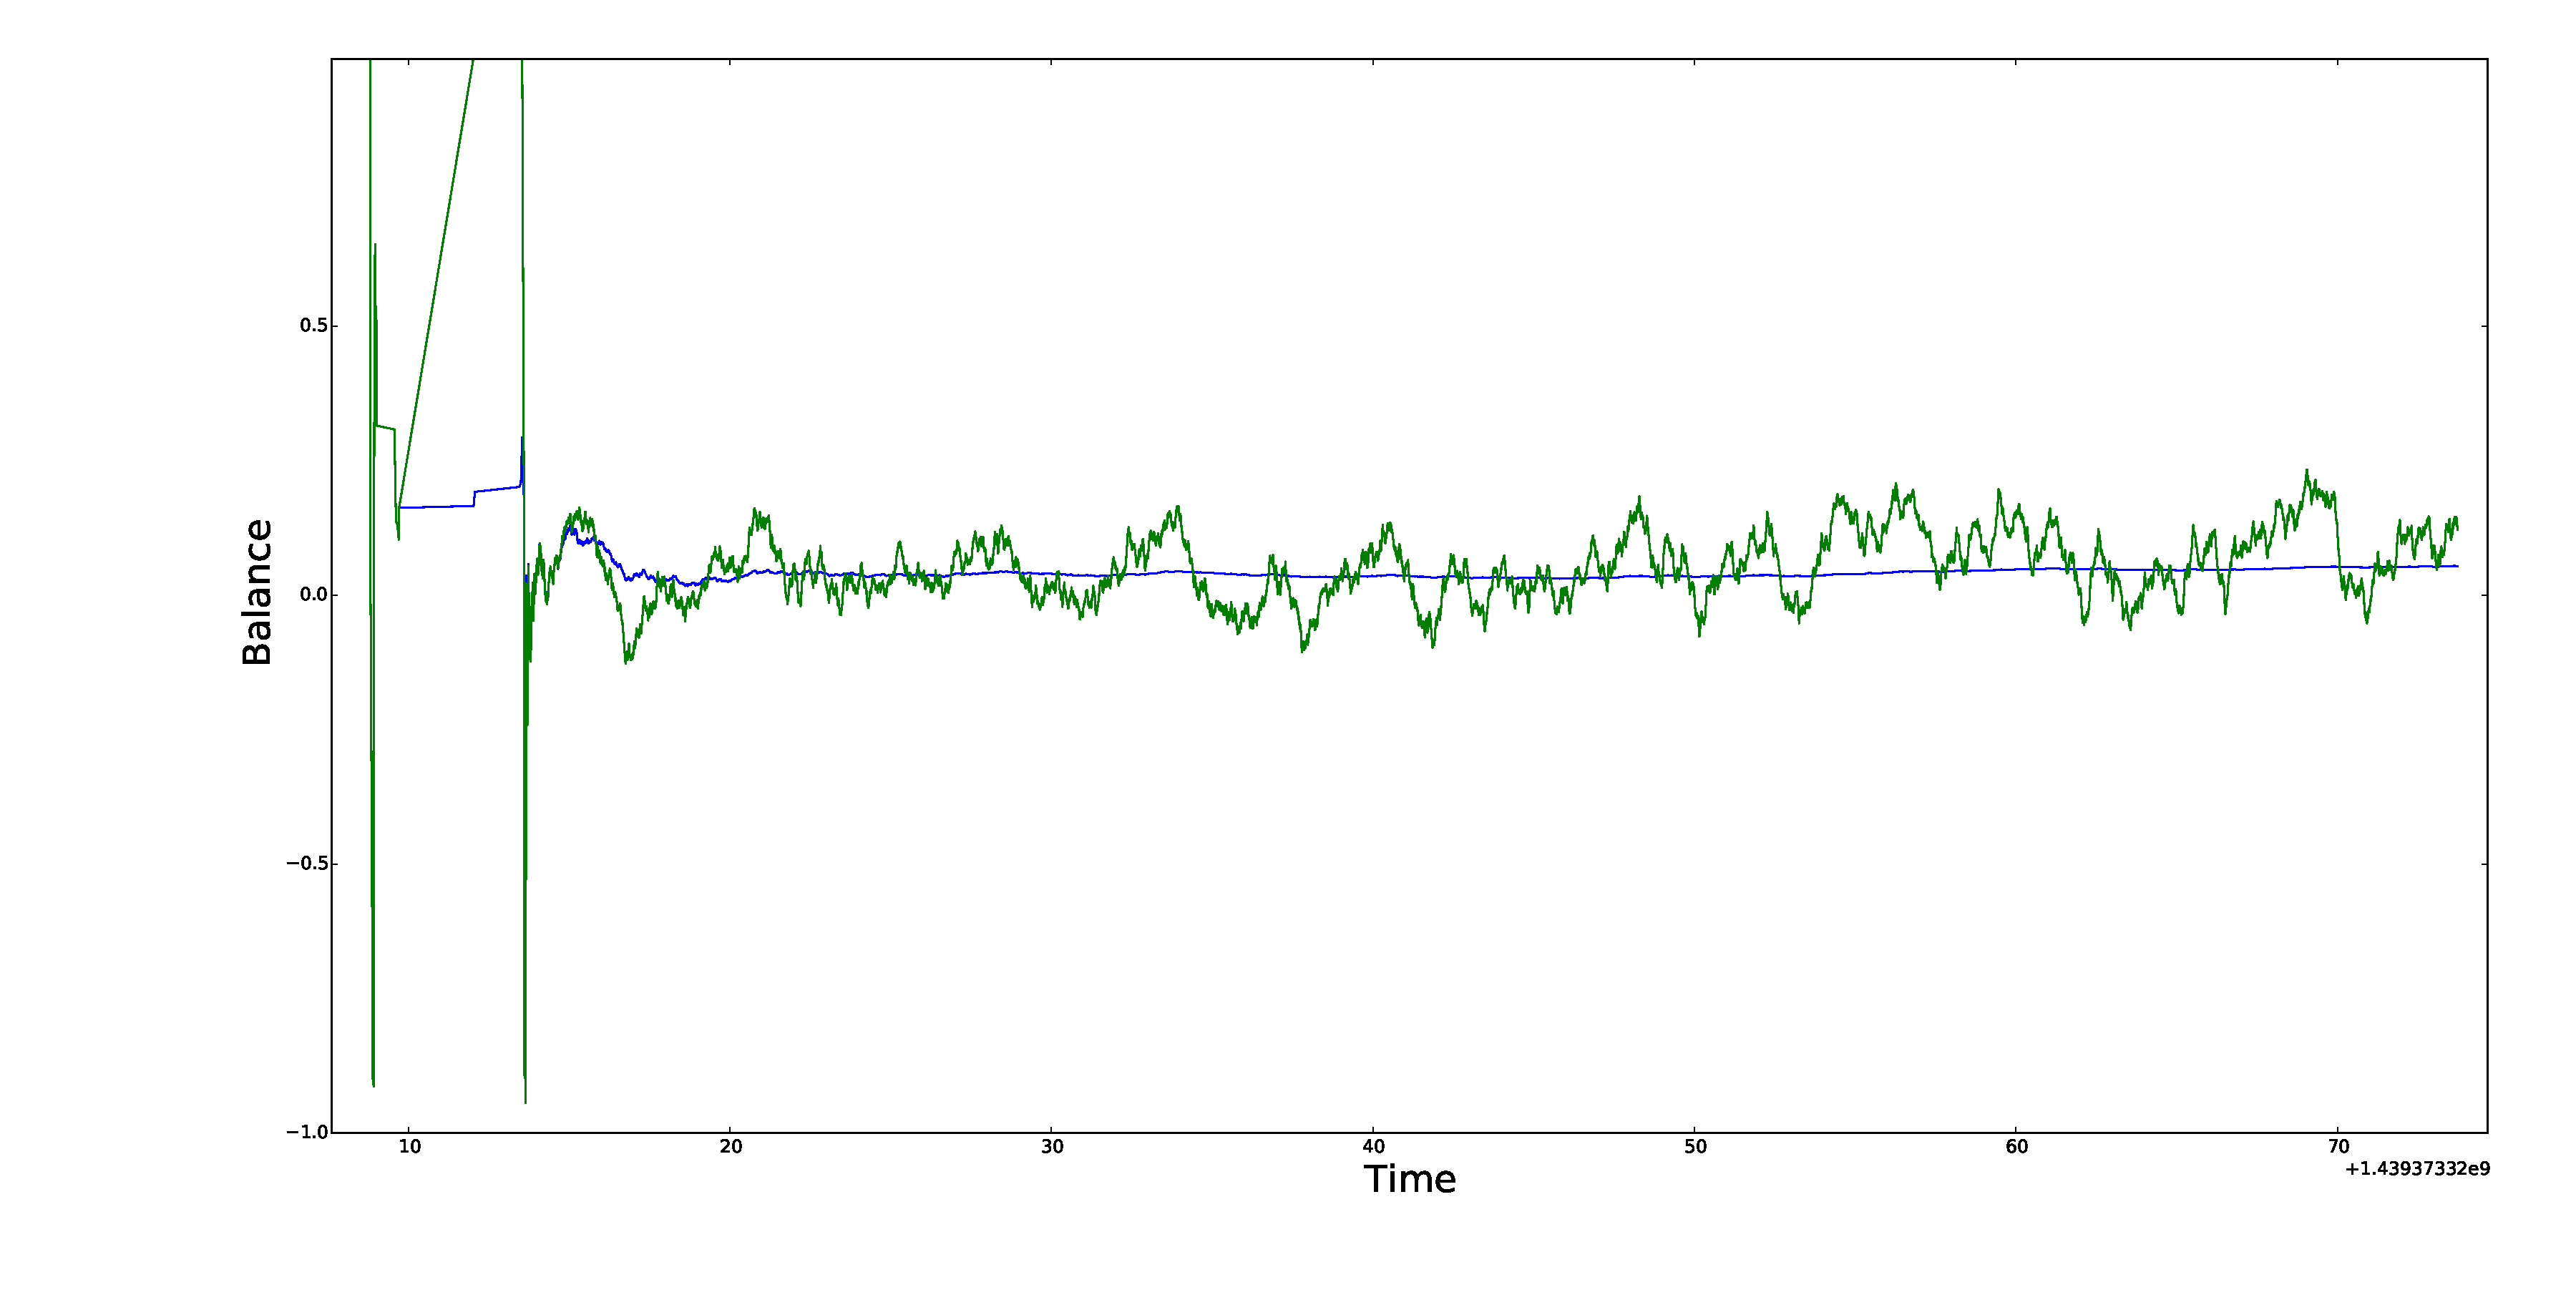
\includegraphics[width=16cm]{../results/subflow_split.pdf}
    \caption{MPTCP Subflows Balance}
    \label{mptcptrace_subflow}
  \end{figure}

  To conclude for this test, even if UDP is faster than TCP in some cases, it should bet taken into account that with UDP if the link fails, the connection is lost.
  Depending on what you are looking for, it can be usefull to have a more robust connection even if it is slower and in that case use TCP.


   \subsection{Delay introduced on links} \label{sec:delay_on_links}

   This section presents the same test than in section \ref{sec:bulk_data_transfer} adding the insertion of delay on links and I then analyse which effect it has on the throughput. The delay are 25ms and 200ms on both links which give a 50RTT and a 400RTT. The buffers sizes are the default OpenVPN buffer size, 64k.

On figure \ref{tcp_vs_udp_200ms} the effect of delay on the througput using TCP and UDP as OpenVPN protocol is presented

\begin{itemize}
\item For TCP the OpenVPN buffer size (64k) is a real disaster and the overall speed is very low compared to the 2ms RTT (see figure \ref{all_tcp_vs_udp}).
\item For UDP he OpenVPN buffer size is not as bad as for TCP but the overall speed still decrease a lot.
\end{itemize}

For TCP this is mainly caused by wrong buffer size. Indeed the computation of the maximum throughput possible with a buffer of 64k and a RTT of 400ms
is obtain 1.3Mbit/s. The same computation for a RTT of 50ms is 10Mbit/s. This is show on figure \ref{tcp_vs_udp_200ms}.

Figure \ref{window_tcp_32_50_full} is the windows graph created by mptcp for the link bandwith of 32mbit/s with a RTT of 400ms. You can see that the window is totally full.

\begin{figure}[h!]
 \centering
 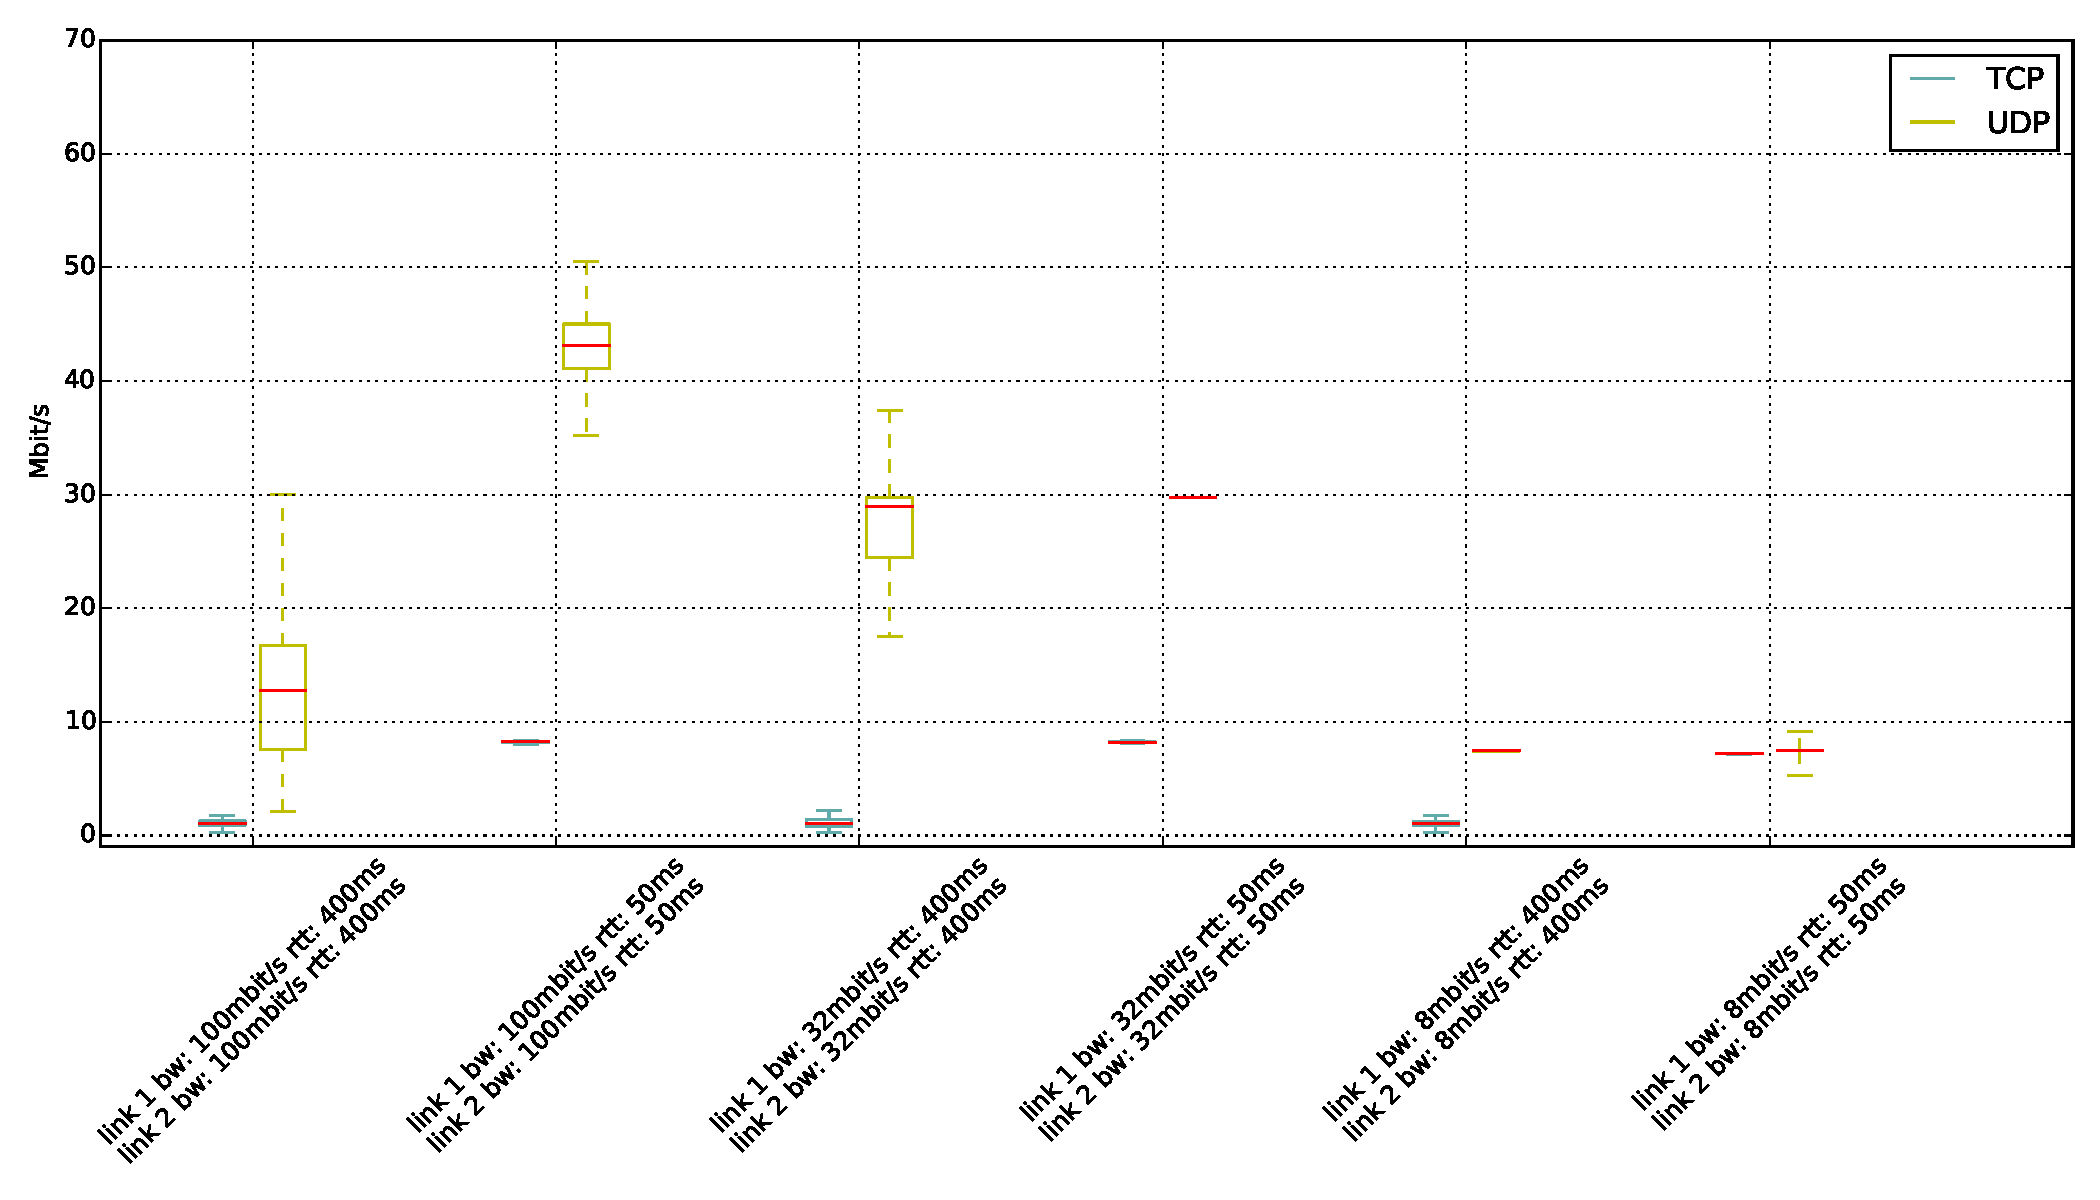
\includegraphics[width=1\textwidth]{../results/all_tcp_vs_udp_200ms.pdf}
 \caption{TCP vs UDP with high RTT buffer: 64k}
 \label{tcp_vs_udp_200ms}
\end{figure}

\begin{figure}[h!]
 \centering
 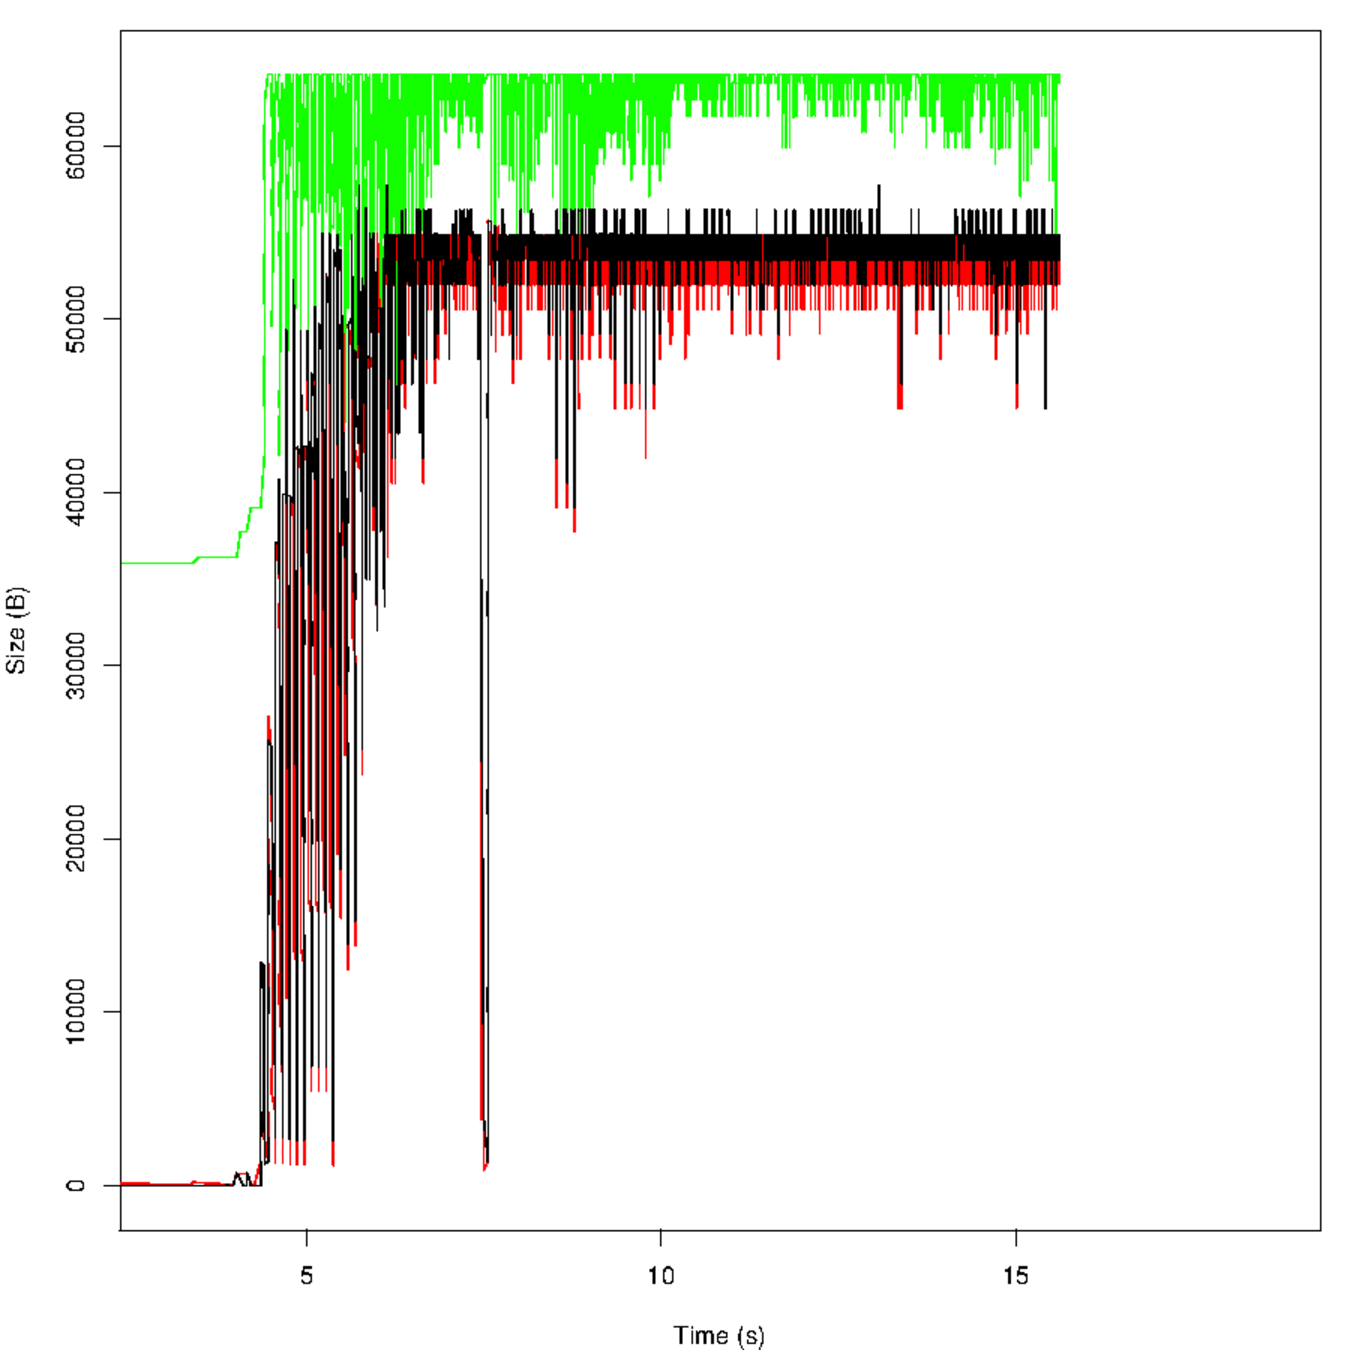
\includegraphics[width=10cm]{../results/window_tcp_32_50_full.pdf}
 \caption{TCP Window being full}
 \label{window_tcp_32_50_full}
\end{figure}

This time the router CPU is around 20\%-30\% usage so there is no bottleneck.
Section \ref{sec:improving_throughput} presents and attempt to resolve this situation by changing buffer size on the openvpn client and openvpn server.

\newpage

\subsection{Request/Response}

In this section I test the number of request / response per second when using TCP or UDP as the OpenVPN protocol. In this purpose I use test from Netperf and Apache Benchmark tool.
My goal is to determine wether a browsing experience for a user would be possible or not depending on the network.

\subsubsection{TCP\_CRR}

  Test setup :

  \begin{itemize}
  \item First link bandwith of 8mbit/s, 32mbit/s, 100mbit/s  and RTT: 2ms, 400ms (default route)
  \item Second link bandwith of 8mbit/s, 32mbit/s, 100mbit/s  and RTT: 2ms, 400ms
  \item Using default mptcp scheduler
  \item OpenVPN buffer default size 65536 bytes on client and server
  \item Congestion control : cubic
  \item Request message size : 1 byte
  \item Response message size : 1 byte
  \end{itemize}

  \begin{figure}[h!]
    \centering
    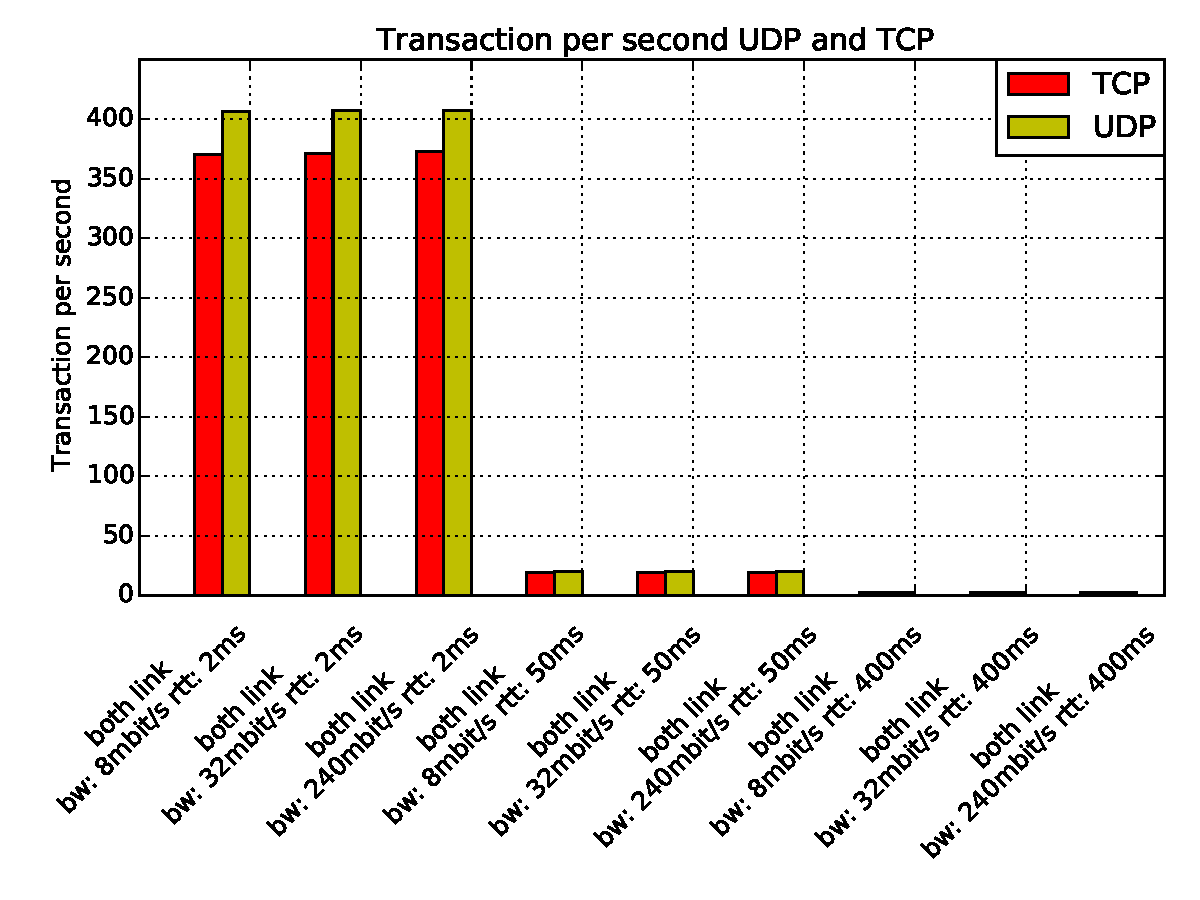
\includegraphics[width=16cm]{../results/tcp_vs_udp_transaction.pdf}
    \caption{TCP vs UDP transaction per second request and response size : 1 byte}
    \label{tcp_vs_udp_transaction}
  \end{figure}

  In this test the CPU and links bandwith do not seems to be the bottleneck. What seems to be the problem is the overhead due to creating and destroying TCP connection for each transaction.

  Figure \ref{tcp_vs_udp_transaction} shows that UDP seems to be a bit better. TCP being a connection-oriented protocol, it takes a bit more time to set up a connection than UDP.
  On top of that, the amount of data to be transmitted inside one transaction is very small, which means that a single connection is destroyed almost immediatly and it creates another one right away,
  this make the connection setup time very impactful.

  In figure \ref{tcp_vs_udp_transaction} is also visible the huge effect of the delay on the number of transaction per second,
  goes up to 400 transaction per second with a RTT of 2ms and it goes down to 2 transaction per second with a RTT of 400ms.

  A high RTT, means that the creation and the teardown of a connection takes more time and because the test are synchronous,
  A transaction has to wait for the previous one transaction to finish before starting.

  Increasing the data transmited into one transaction would be a more realistic and fair test between TCP and UDP.
  I used a 100 bytes request message size and a 170 bytes response message size to have identical size than the test done with Apache Benchmark (see section \ref{sec:ab}).

  \begin{figure}[h!]
    \centering
    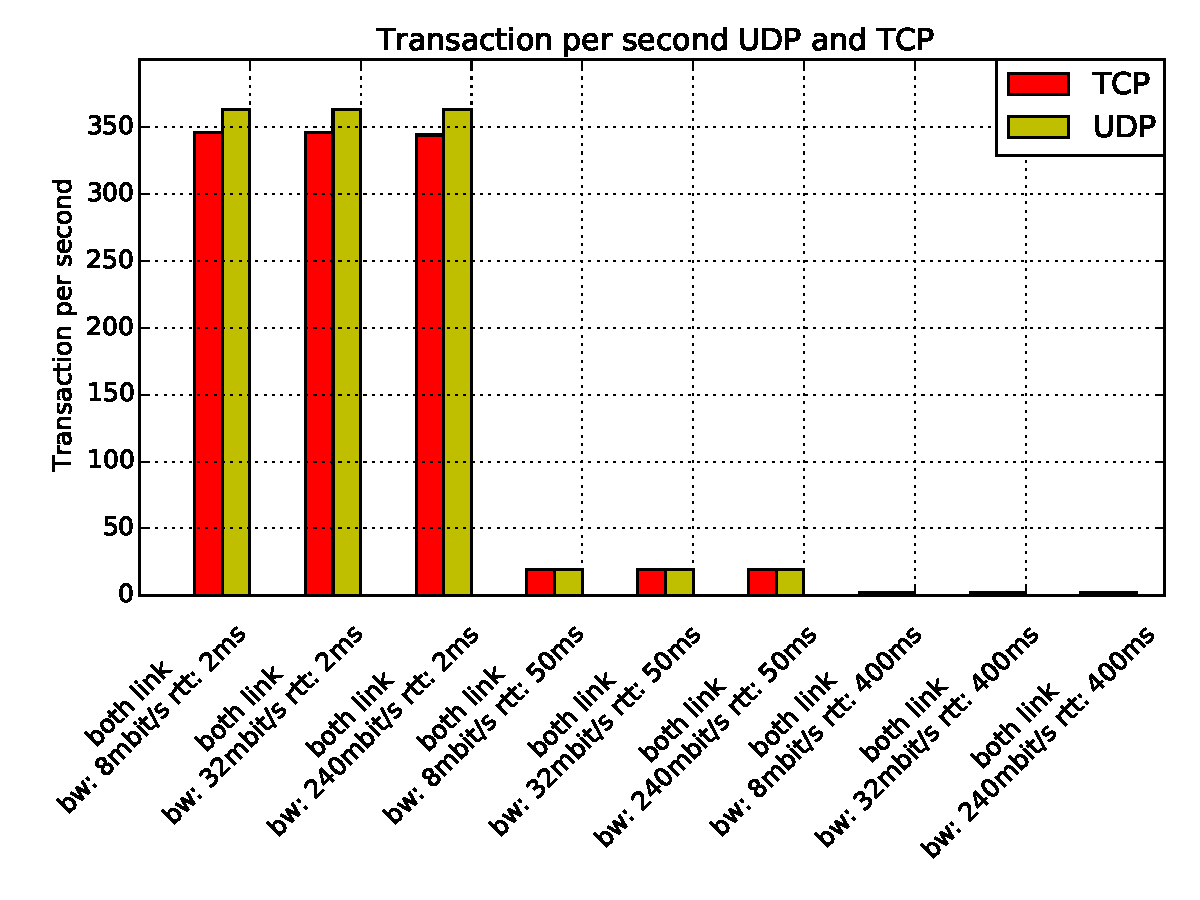
\includegraphics[width=16cm]{../results/tcp_vs_udp_transaction_fair.pdf}
    \caption{TCP vs UDP transaction per second request size : 100 / response size : 170 byte}
    \label{tcp_vs_udp_transaction_fair}
  \end{figure}

  Figure \ref{tcp_vs_udp_transaction_fair} shows that the difference between TCP and UDP is smaller because the data transmitted inside one transaction is bigger and
  the connection setup time has less impact. However the effect of the delay is still very strong and confirm my previous conclusion.

  In conclusion, for this kind of traffic, MPTCP will not improve performance. The advantage of using multiple paths is not very usefull (only if one path fails) because it has no concurrent transaction
  and they are executed synchronously. In this case, UDP seems to be a better choice.

  Hewever these tests might not reflect reality because normaly one would use one TCP connection for multiple transactions
  and  establish multiple connections, unfortunatly Netperf does not provide such a test. To do that I use Apache Benchmark see section \ref{sec:ab} below.

\subsubsection{Apache Benchmark (AB)} \label{sec:ab}

The choice to run AB is to provide a more realistic way to test the process of request\/response to a real web server.
It also gives the possibility to use simultanious connections with the http \textit{keep-alive} option.

When \textit{keep-alive} option is set to true, it uses a single TCP connection to send and receive multiple HTTP request/response,
as opposed to opening a new connection for every single request/response transaction like in TCP\_CCR from netperf.

The settings used to run AB are :

\begin{itemize}
\item 6 concurrent connections, usually browser use between 6(Firefox,Chrome) and 8(Opera)
\item maximum time of 60 seconds
\item option \textit{keep-alive} enable
\end{itemize}

AB always stops after 50000 transaction even if the total time has not been totaly spent.
The requests made by AB have a size of 100 bytes and the responses by the Apache server have a size of 170 bytes.

   \begin{figure}[h!]
    \centering
    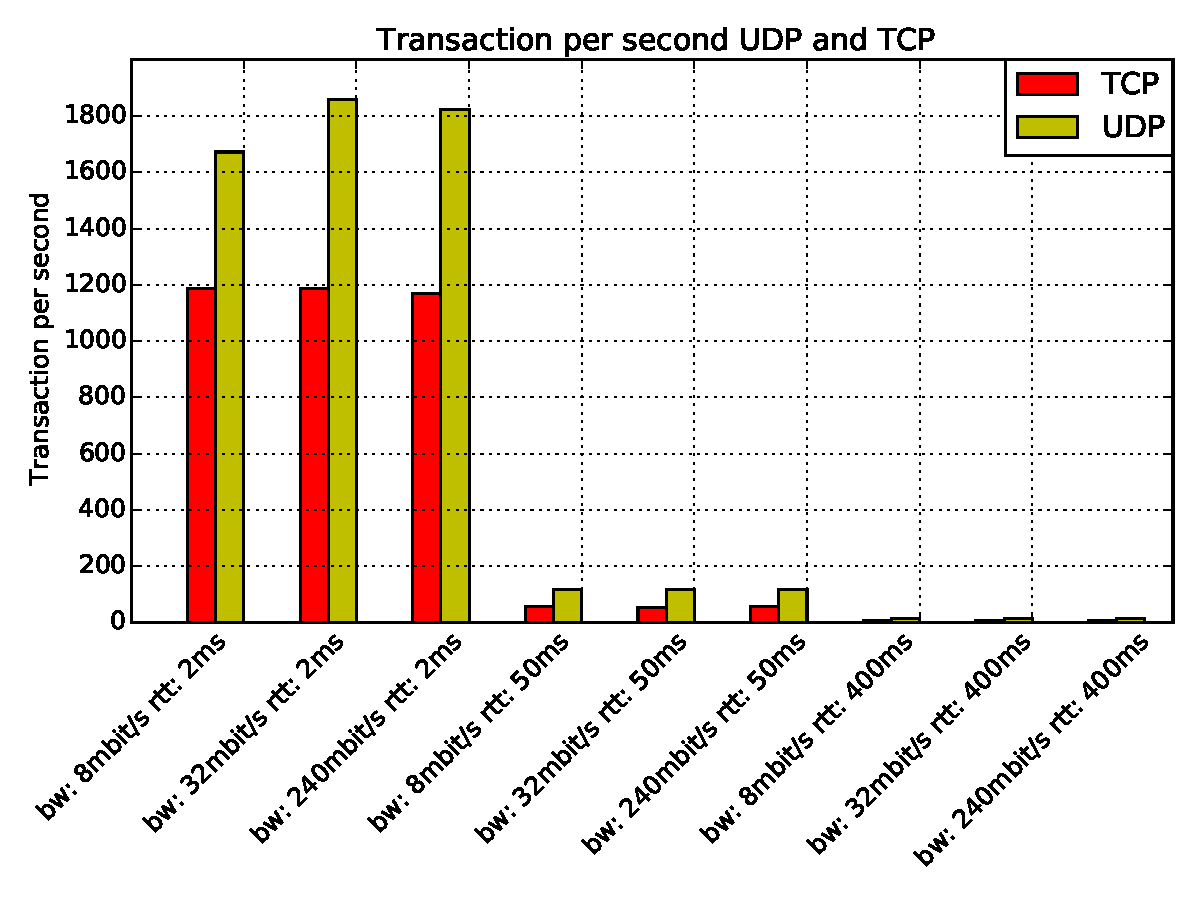
\includegraphics[width=1\textwidth]{../results/all_request_response_ab.pdf}
    \caption{Request/Response Apache benchmark}
    \label{all_request_response_ab}
  \end{figure}

Figure \ref{all_request_response_ab} shows that the number of transactions with UDP and TCP using apache benchmark. The number are quite bigger than the one from the previous tests TCP\_CRR.
The maximum is 1800 transactions per second when using UDP and a RTT of 2ms. The minimum is 6 transactions per second when using TCP and having a RTT of 400ms.

The links maximum bandwith do not have a big impact on the number of transaction per second, it is
mainly the RTT. In this test UDP still dominate even with the concurrent connections being used.

It is the same as the TCP\_CRR test: the CPU and link bandwith are not the bottle neck,
the CPU usage of the router is around 25-30\% during the tests. The problem is the time it takes to establish a connection when using TCP.

In conclusion, TCP gives reasonnable performances compared to UDP and This leads me to think that it could be used without impacting too much on the user experience.

New, I look at what happen if the main link fails during a certain span of time to evaluate wether in this case MPTCP has the advantage.

The test length is 30 second and the main link will be set to 100\% packet loss after 5 seconds and then set back to 0\% after 15 seconds.
The links RTT are 2ms and max bandwidth is 8mbit/s and 32mbit/s.

On figure \ref{request_response_link_down_ab}, we see that this time the difference between the transaction per second for UDP and TCP is smaller because TCP continue to transmit data while
UDP is stopped.

Inserting more down time on the link makes this behavior even more visible and UDP is slower than TCP.
This is because MPTCP switches the traffic to another subflow when it finds out that the one it is using starts to have timeout.
UDP however cannot do that and will not be able to transmit data during this time.

   \begin{figure}[h!]
    \centering
    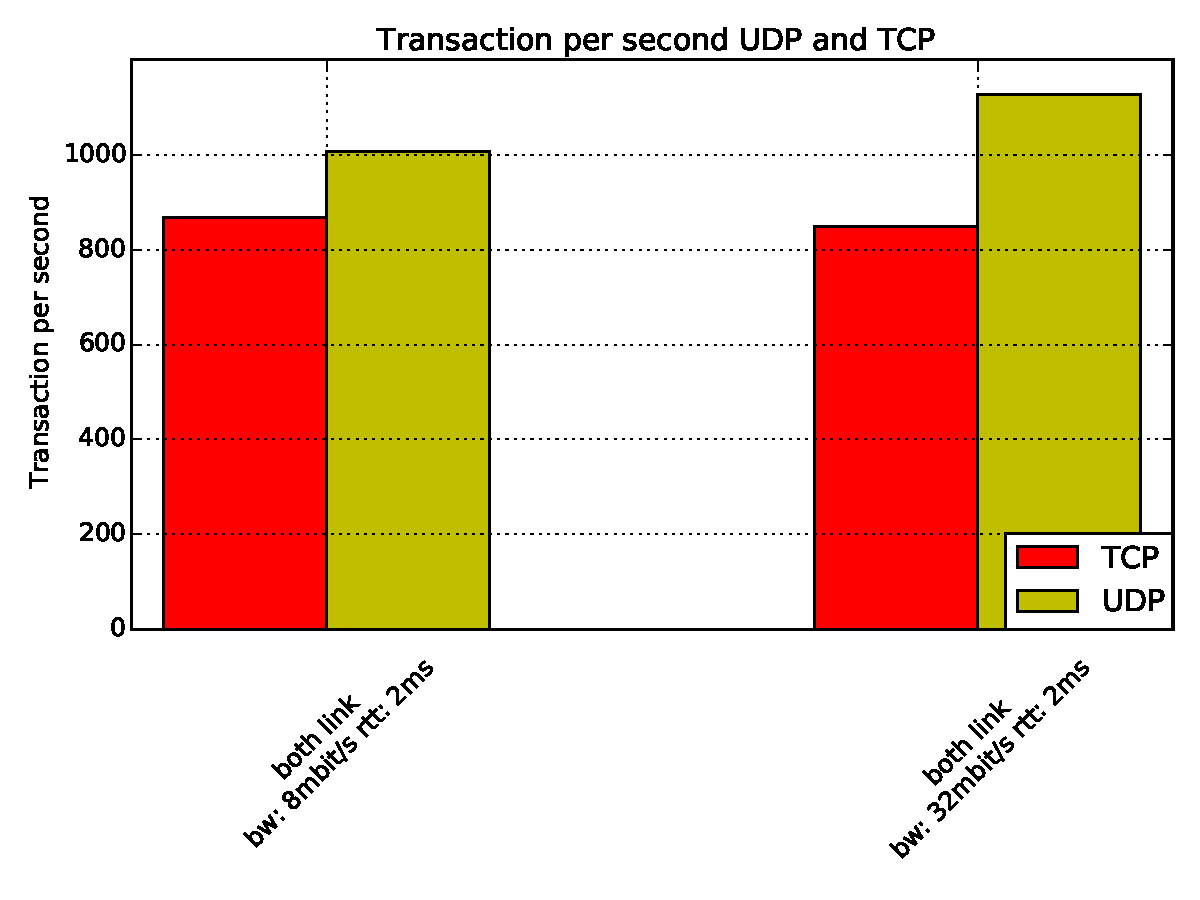
\includegraphics[width=8cm]{../results/request_response_link_down_ab.pdf}
    \caption{Request/Response Apache benchmark one link down}
    \label{request_response_link_down_ab}
  \end{figure}

   \begin{figure}[h!]
    \centering
    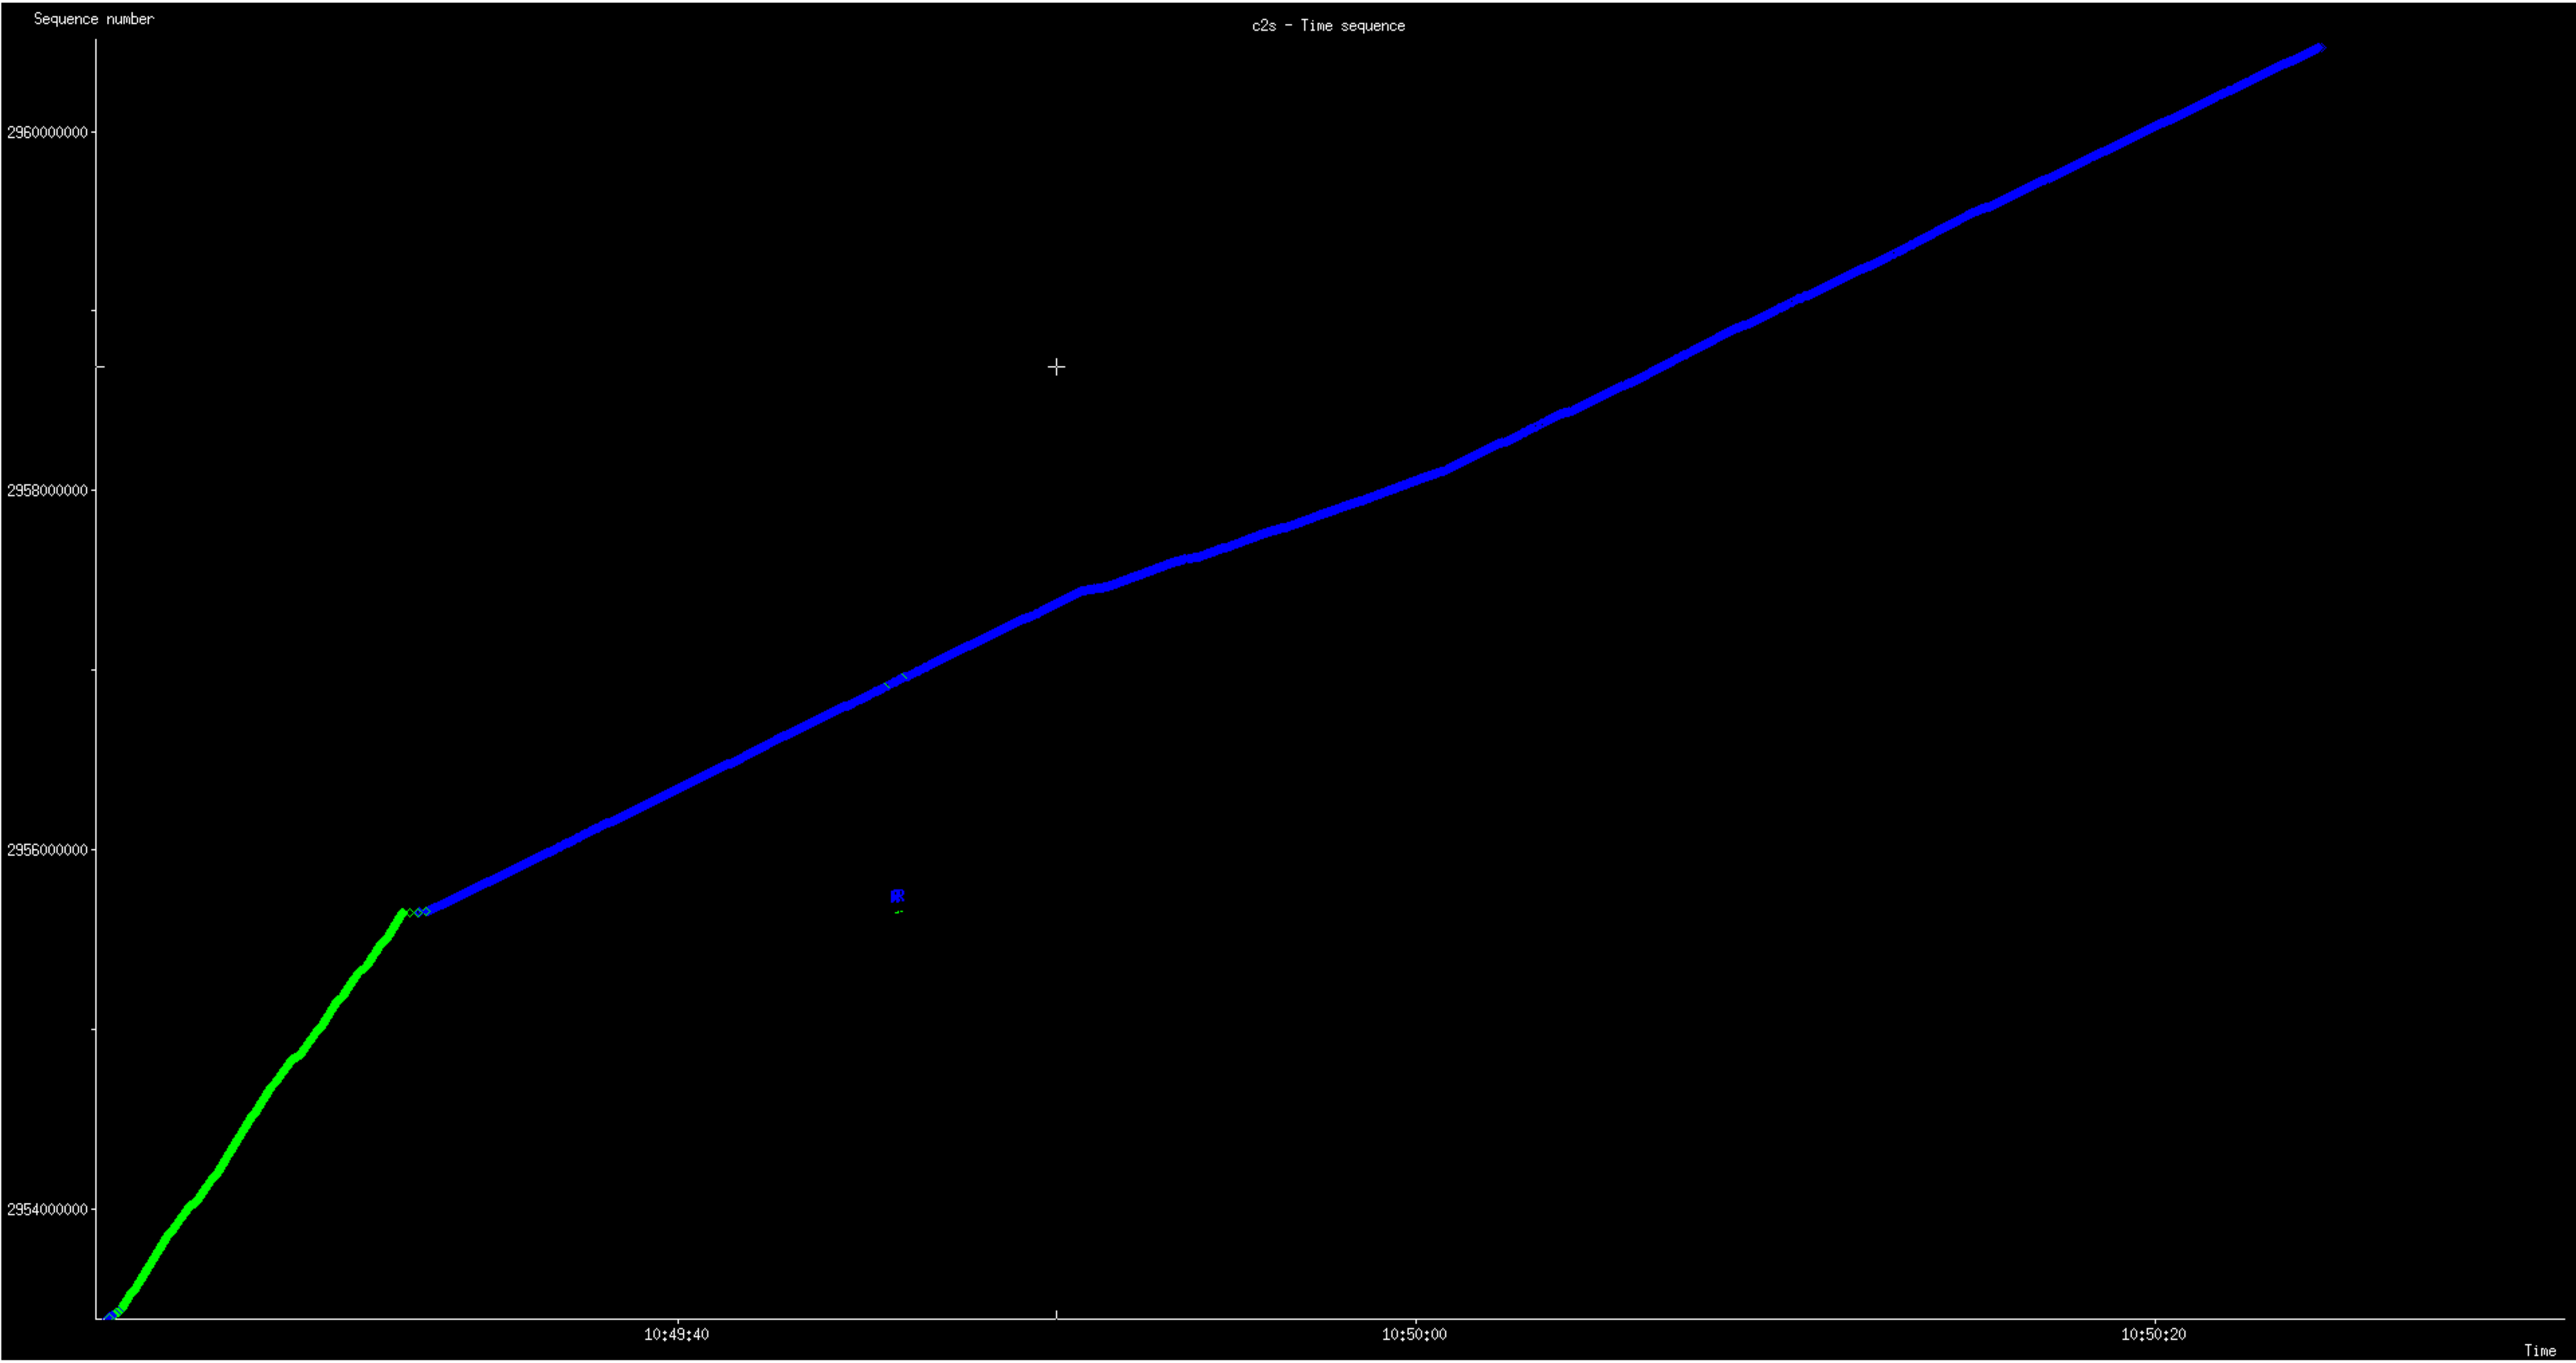
\includegraphics[width=8cm]{../results/request_response_subflow_change.pdf}
    \caption{Request/Response Apache benchmark one link down subflow details}
    \label{request_response_subflow_change}
  \end{figure}


Figure \ref{request_response_subflow_change} is the sequence number graph of the MPTCP connection.
It presents the switch from the main subflow (the green line) to the alternative subflow (the blue line) when the link goes down.

\section{Links with different bandwidth and delay}

For these tests I go back to builk data transfer test and I look at the impact on the throughput when using links with different bandwith and delay.
Here I only use TCP has OpenVPN protocol. UDP is not very interesting because it only uses one link.

This is interesting because we will see how MPTCP decides to split traffic on the two subflows depending on their RTT and their bandwidth.

\subsection{First test setup} \label{sec:first_test}

\begin{itemize}
\item First link bandwith of 32mbit/s and RTT: 2ms (default route)
\item Second link bandwith of 8mbit/s and a RTT: 2ms
\item Using default mptcp scheduler
\item OpenVPN buffer set to 64000 byte (TCP windows size) on client and server
\item Congestion control : cubic
\end{itemize}

In theory we would like to get around 40mbit/s of throughput. In practice we get a 35mbit/s througput, the router is not the bottleneck the CPU is utilized around 60\%.

This setup will be used for further tests in section \ref{sec:improving_throughput_congestion_control}

\subsection{Second test setup}

\begin{itemize}
\item First link bandwith of 32mbit/s and RTT: 2ms (default route)
\item Second link bandwith of 8mbit/s and a RTT: 400ms
\item Using default MPTCP scheduler
\item OpenVPN buffer set to 400000 byte (TCP windows size) on client and server
\item Congestion control : cubic
\end{itemize}

In theory we would expect a throughput around 40mbit/s which is the sum of the two link Bandwith.

In practice MPTCP only uses the link with the lowest RTT and does not use the second link, this gives a throughput around 30mbit/s.

To analyse how the traffic splits accross the two subflows I use MPTCPtrace to generate the sequence number graph and a script provided by Benjamin Hesmans to generate figure \ref{32_8-2_400rtt_seq}.
On this figure the balance is close to the +1 limit meaning that the traffic is mainly on first subflow (first link) and the second subflow (second link) is rarely used.

The analyse of the sequence graph (not presented) shows that because of the high RTT on the second subflow, packets send on this subflow, are reinjected on the first subflow.

\begin{figure}[h!]
 \centering
 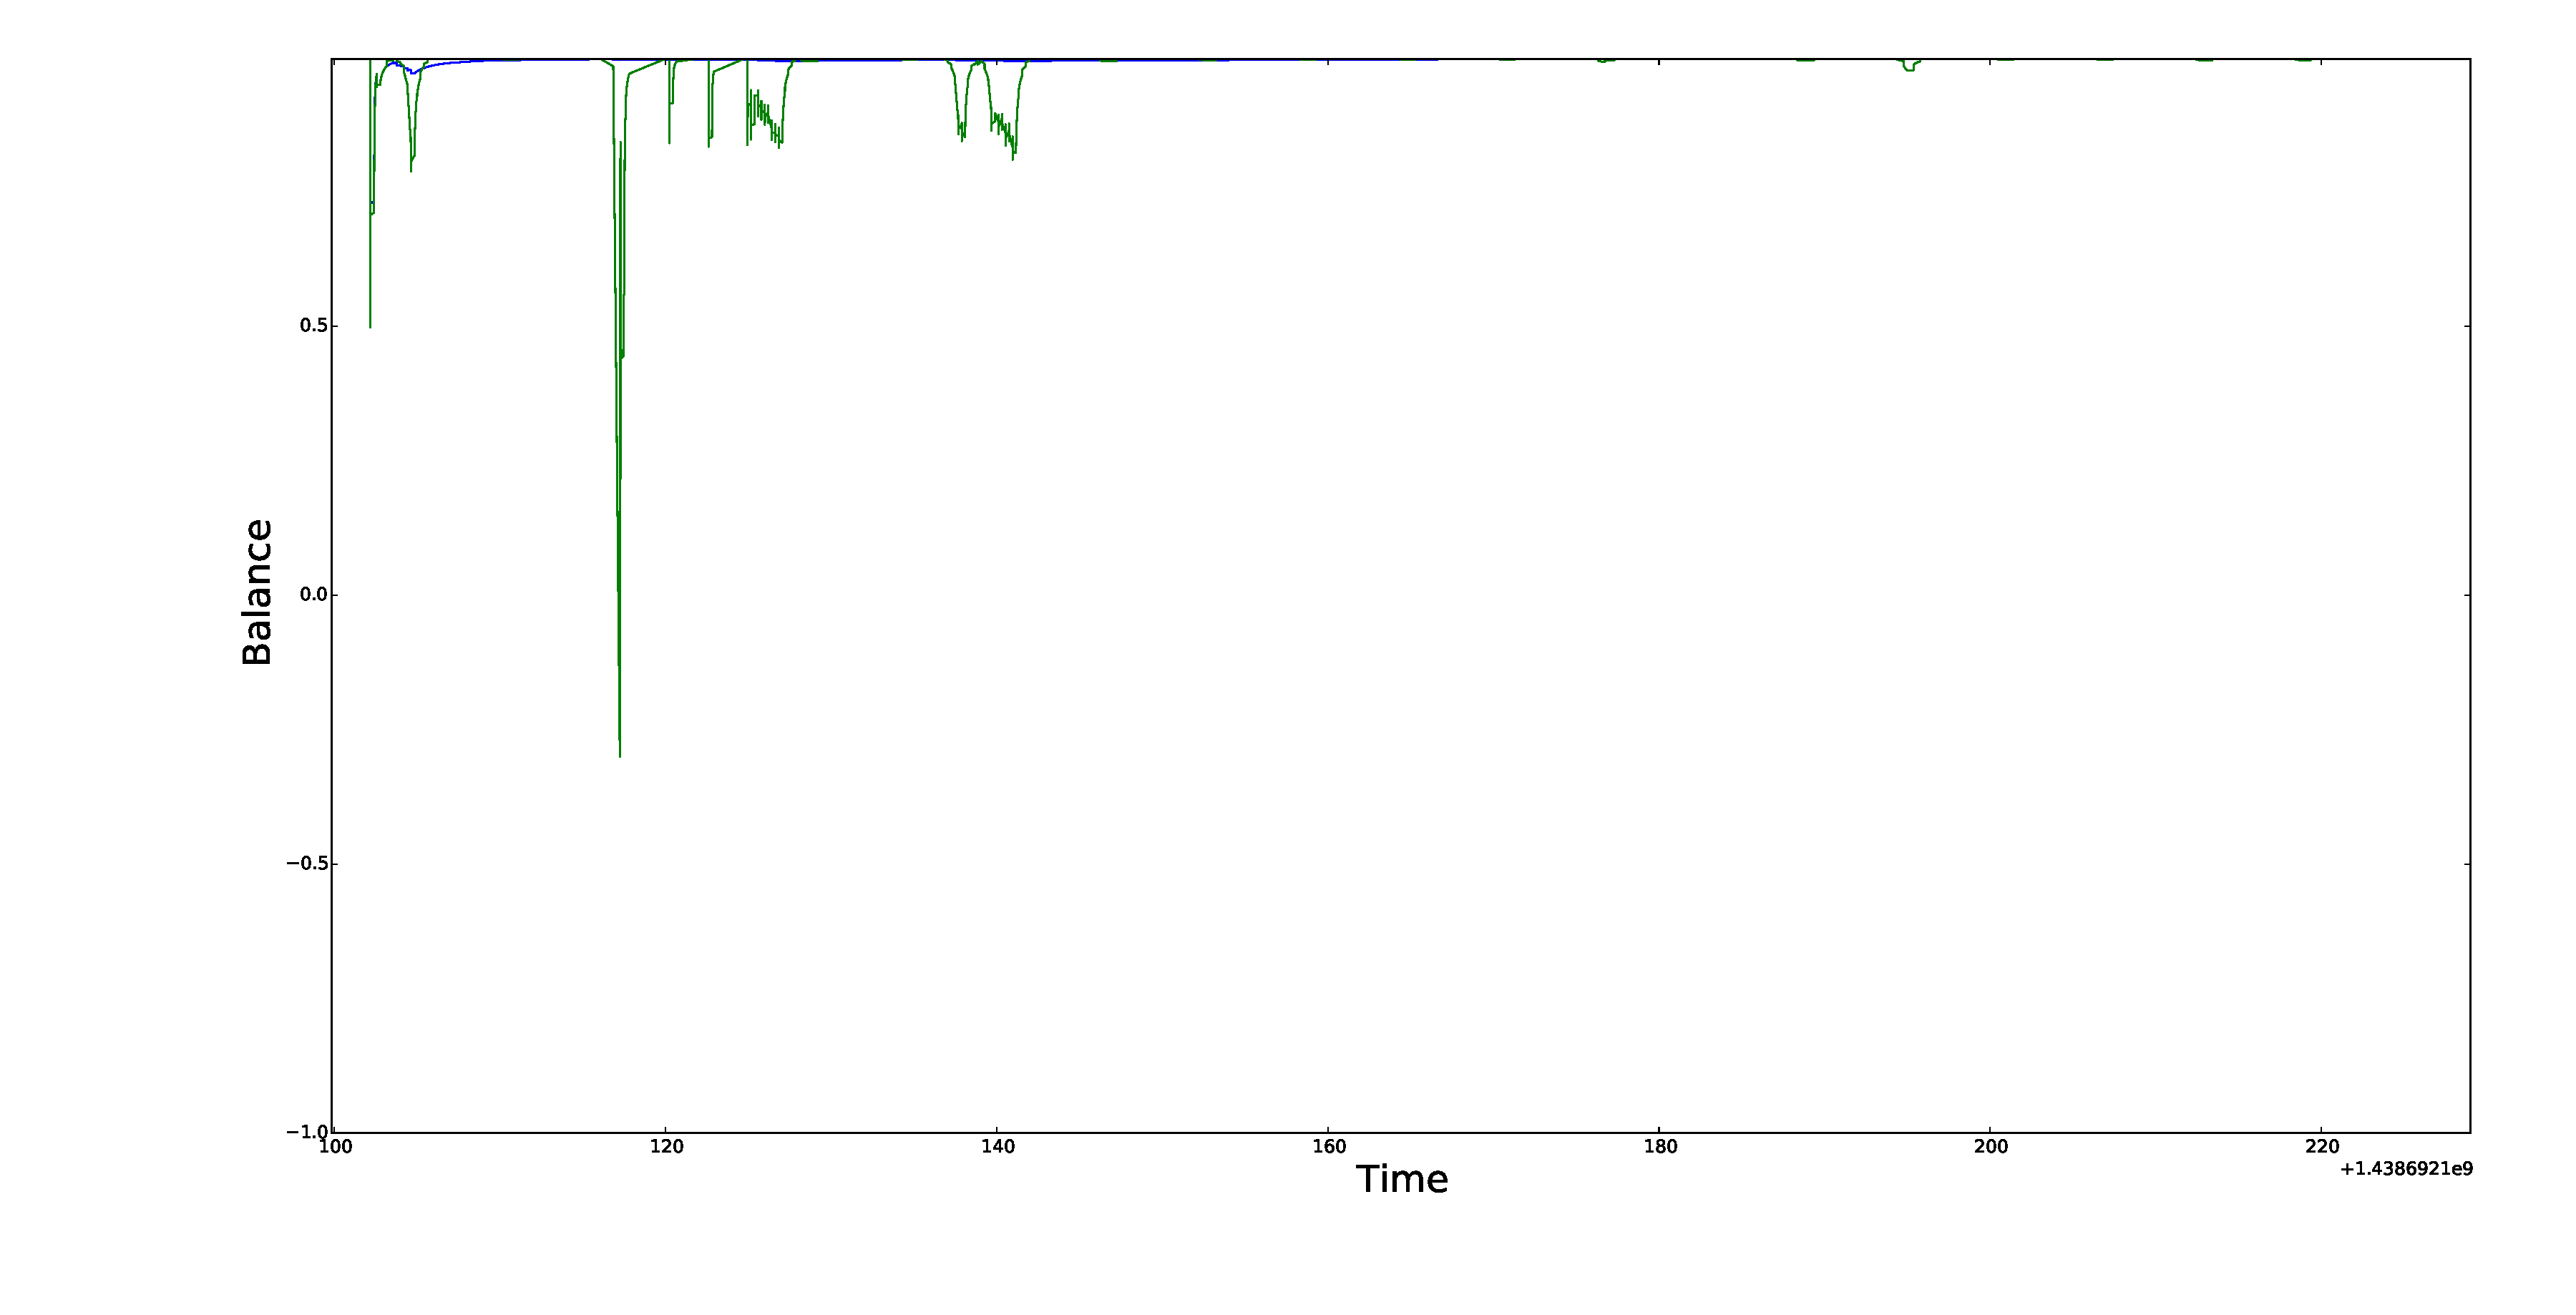
\includegraphics[width=14cm]{../results/32_8-2_400rtt_seq2.pdf}
 \caption{Subflow usage graph second test setup}
 \label{32_8-2_400rtt_seq}
\end{figure}

\subsection{Third test setup} \label{sec:third_test}

\begin{itemize}
\item First link bandwith of 32mbit/s and RTT: 400ms (default route)
\item Second link bandwith of 8mbit/s and RTT: 2ms
\item Using default MPTCP scheduler
\item OpenVPN buffer set to 1600000 byte (TCP windows size) on client and server
\item Congestion control : cubic
\end{itemize}

\begin{figure}[h!]
 \centering
 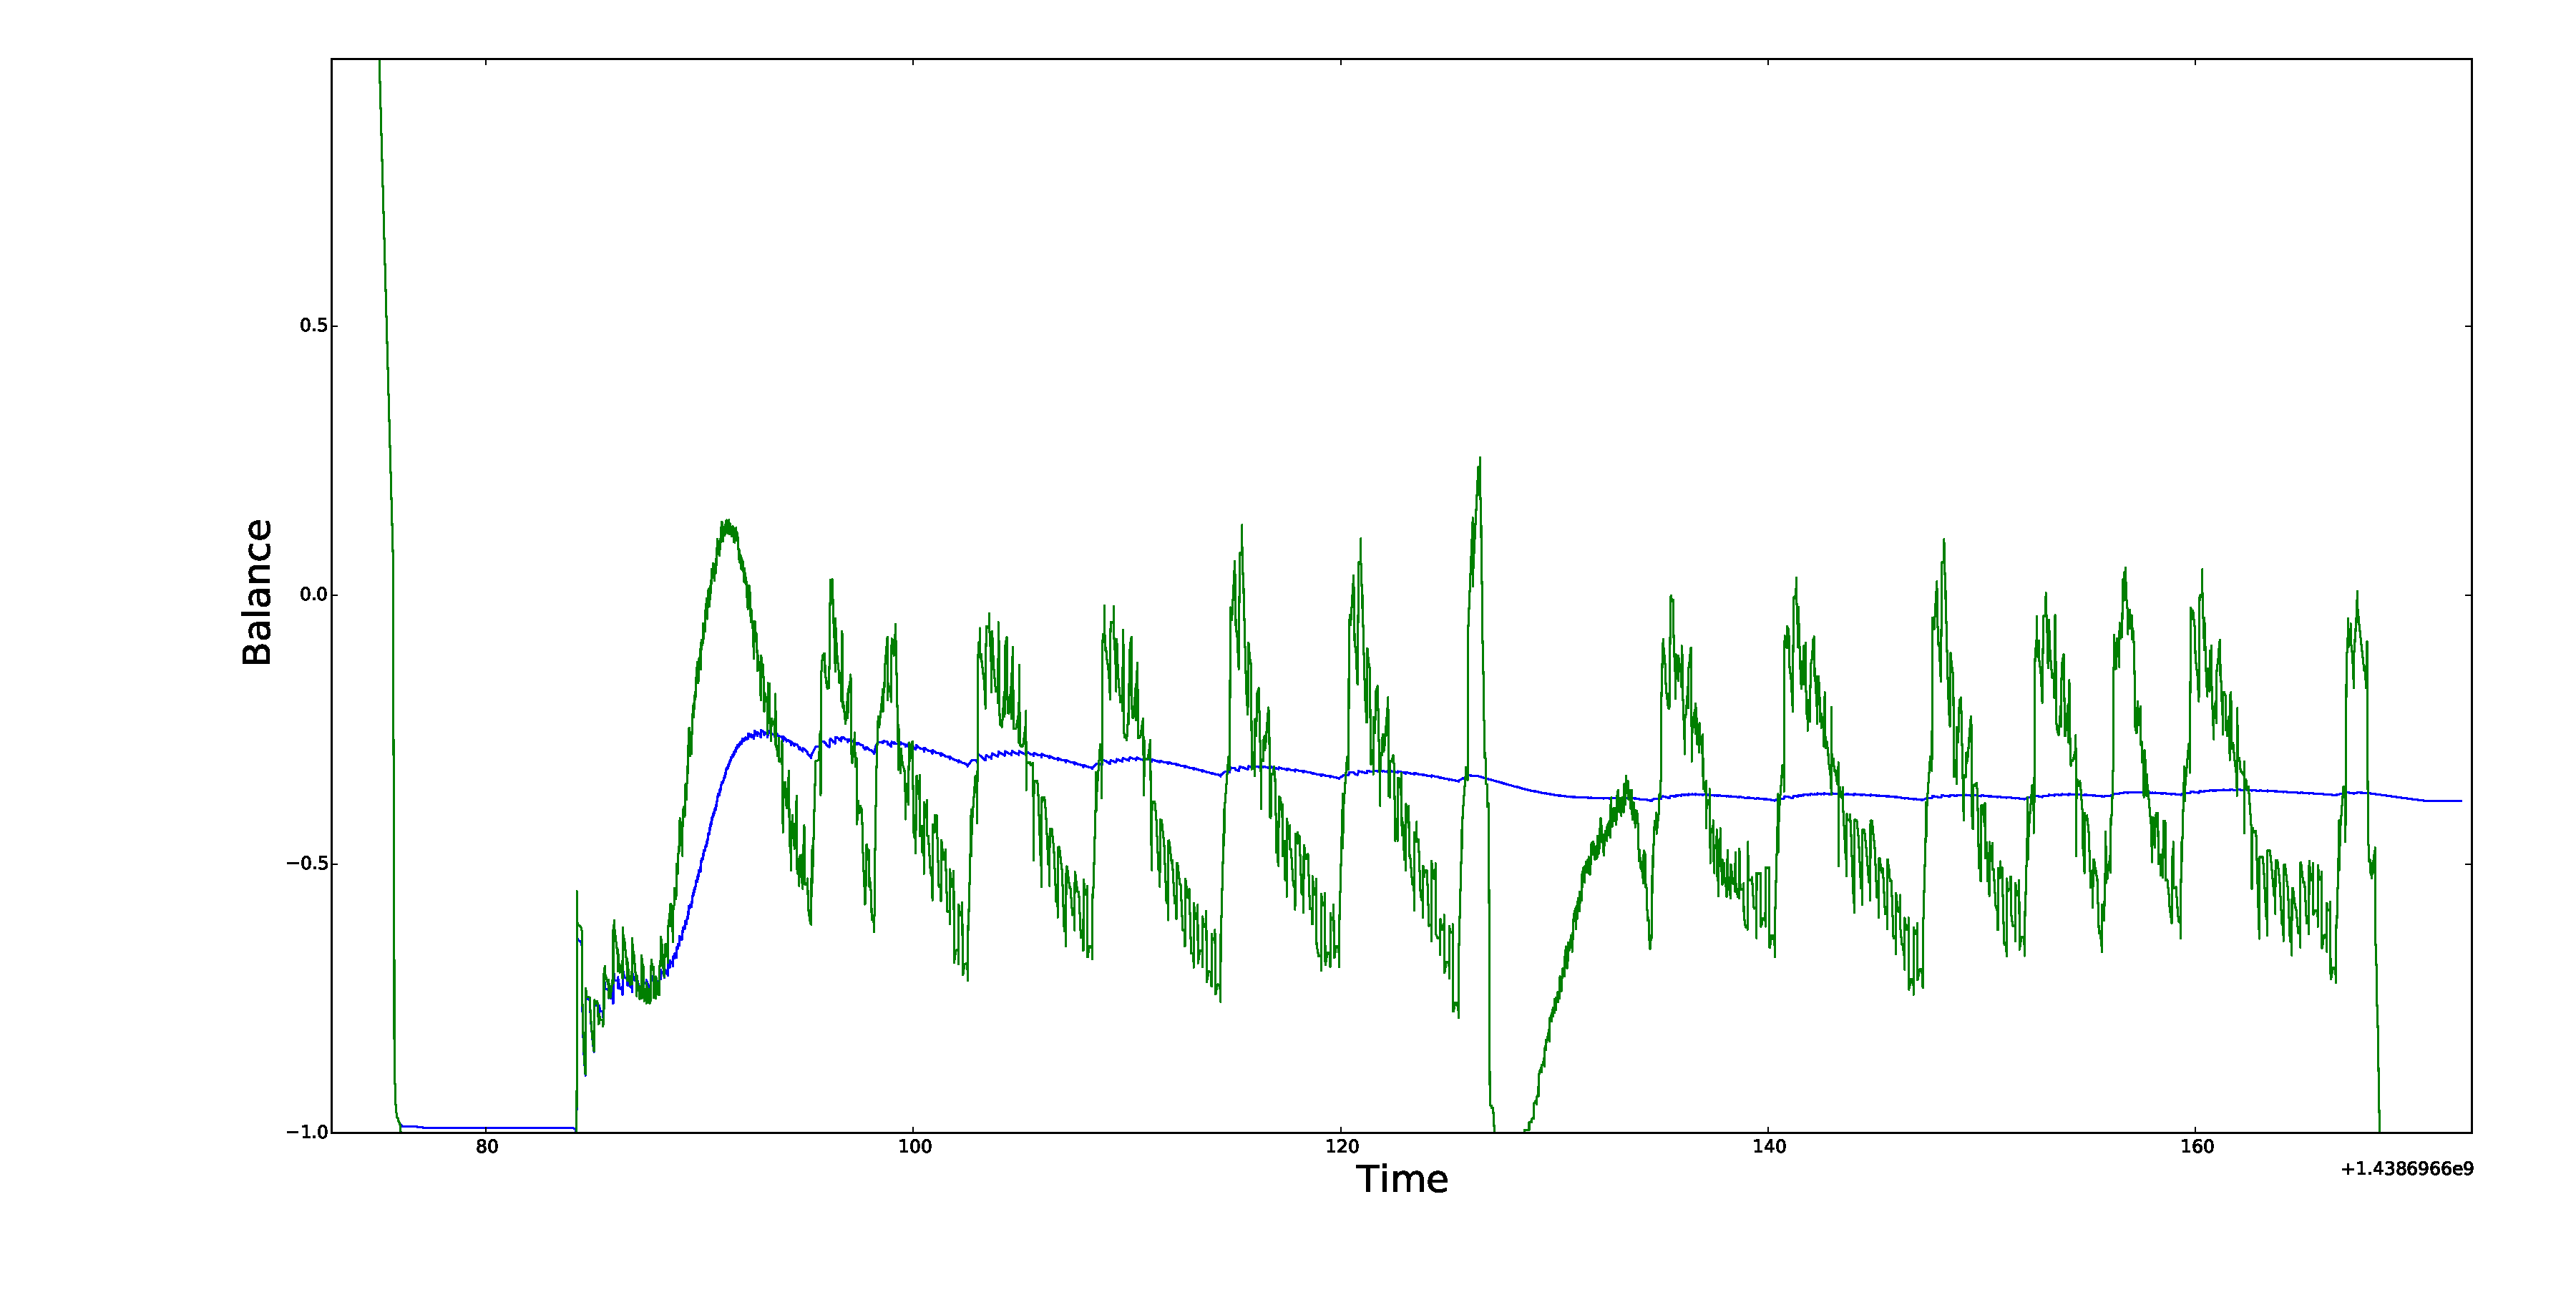
\includegraphics[width=14cm]{../results/32_8-400_2rtt_seq2.pdf}
 \caption{Subflow usage graph third test setup}
 \label{32_8-400_2rtt_seq}
\end{figure}

Here MPTCP use both links but the throughput is only around 8mbit/s. Figure \ref{32_8-400_2rtt_seq} shows that it uses the second subflow (second link) in blue and
 also the first subflow (first link) quite often.

If we look at the sequence graph (not presented) we see that it retransmit some packet from the first subflow to the second subflow because of the high RTT of the first subflow.

In conclusion for some of these setups MPTCP are not optimal and there is room for improvement.
In section \ref{sec:improving_throughput_congestion_control} and \ref{sec:improving_throughput_scheduler}
I will use differents congestion control algorithms and a alternative MPTCP scheduler and check wether it is more adequate.


 \chapter{Improving performance}
 \section{Improving throughput by changing buffer size} \label{sec:improving_throughput}

In previous test \label{sec:delay_on_links} we saw that using the same bandwith but introducing high delay on links decrease the throughput significantly.
This is likely to be due to wrong buffer size more precisely TCP window size.
In this section we will try to adjust buffer size and see if it improves  the results.
I will only use TCP as the OpenVPN protocol because UDP is not my main focus here.

To adjust the TCP maximum send and receive window size, I will set value of \textit{sndbuf} and \textit{rcvbuf} in the openvpn configuration.
To compute the size I will be using the formula : $$(2 * delay * bandwidth) * 2$$.

First I will try on one specific setup from test \ref{sec:delay_on_links}, the 8mbit/s bandwidth limit and 400 RTT.

Now lets use a buffer size of 800000 bytes (390 kbytes) instead of the default one used by openvpn (64kbytes)

This is done by modifying the openvpn configuration file of client and server see \ref{lst:set_buffer_size_openvpn}:

  \begin{lstlisting}[caption={Set buffer size OpenVPN configuration},label={lst:set_buffer_size_openvpn}]
	proto tcp
	sndbuf 800000
	rcvbuf 800000\end{lstlisting}

And modify the maximum buffer size that applications can request by changing /proc/sys/net/core/rmem\_max and /proc/sys/net/core/wmem\_max on the onpenvpn client and
openvpn server~\cite{tcptuning}. You might also have to change the /proc/sys/net/ipv4/tcp\_wmem and /proc/sys/net/ipv4/tcp\_rmem if they are not big enough.(see \ref{lst:set_buffer_size_os})

\begin{lstlisting}[caption={Set max buffer size},label={lst:set_buffer_size_os}]
sysctl -w net.core.wmem_max=800000
sysctl -w net.core.rmem_max=800000
sysctl -w net.ipv4.tcp_rmem='4096	87380	6291456'
sysctl -w net.ipv4.tcp_wmem='4096 16384	4194304'\end{lstlisting}

This gives a 10mbit/s throughput and an average RTT of 450 (see figure \ref{tcp_all_custom_buffer}). This is obviously a better result than the 2mbit/s throughput seen on figure \ref{tcp_vs_udp_200ms}.

  \begin{figure}[h!]
    \centering
    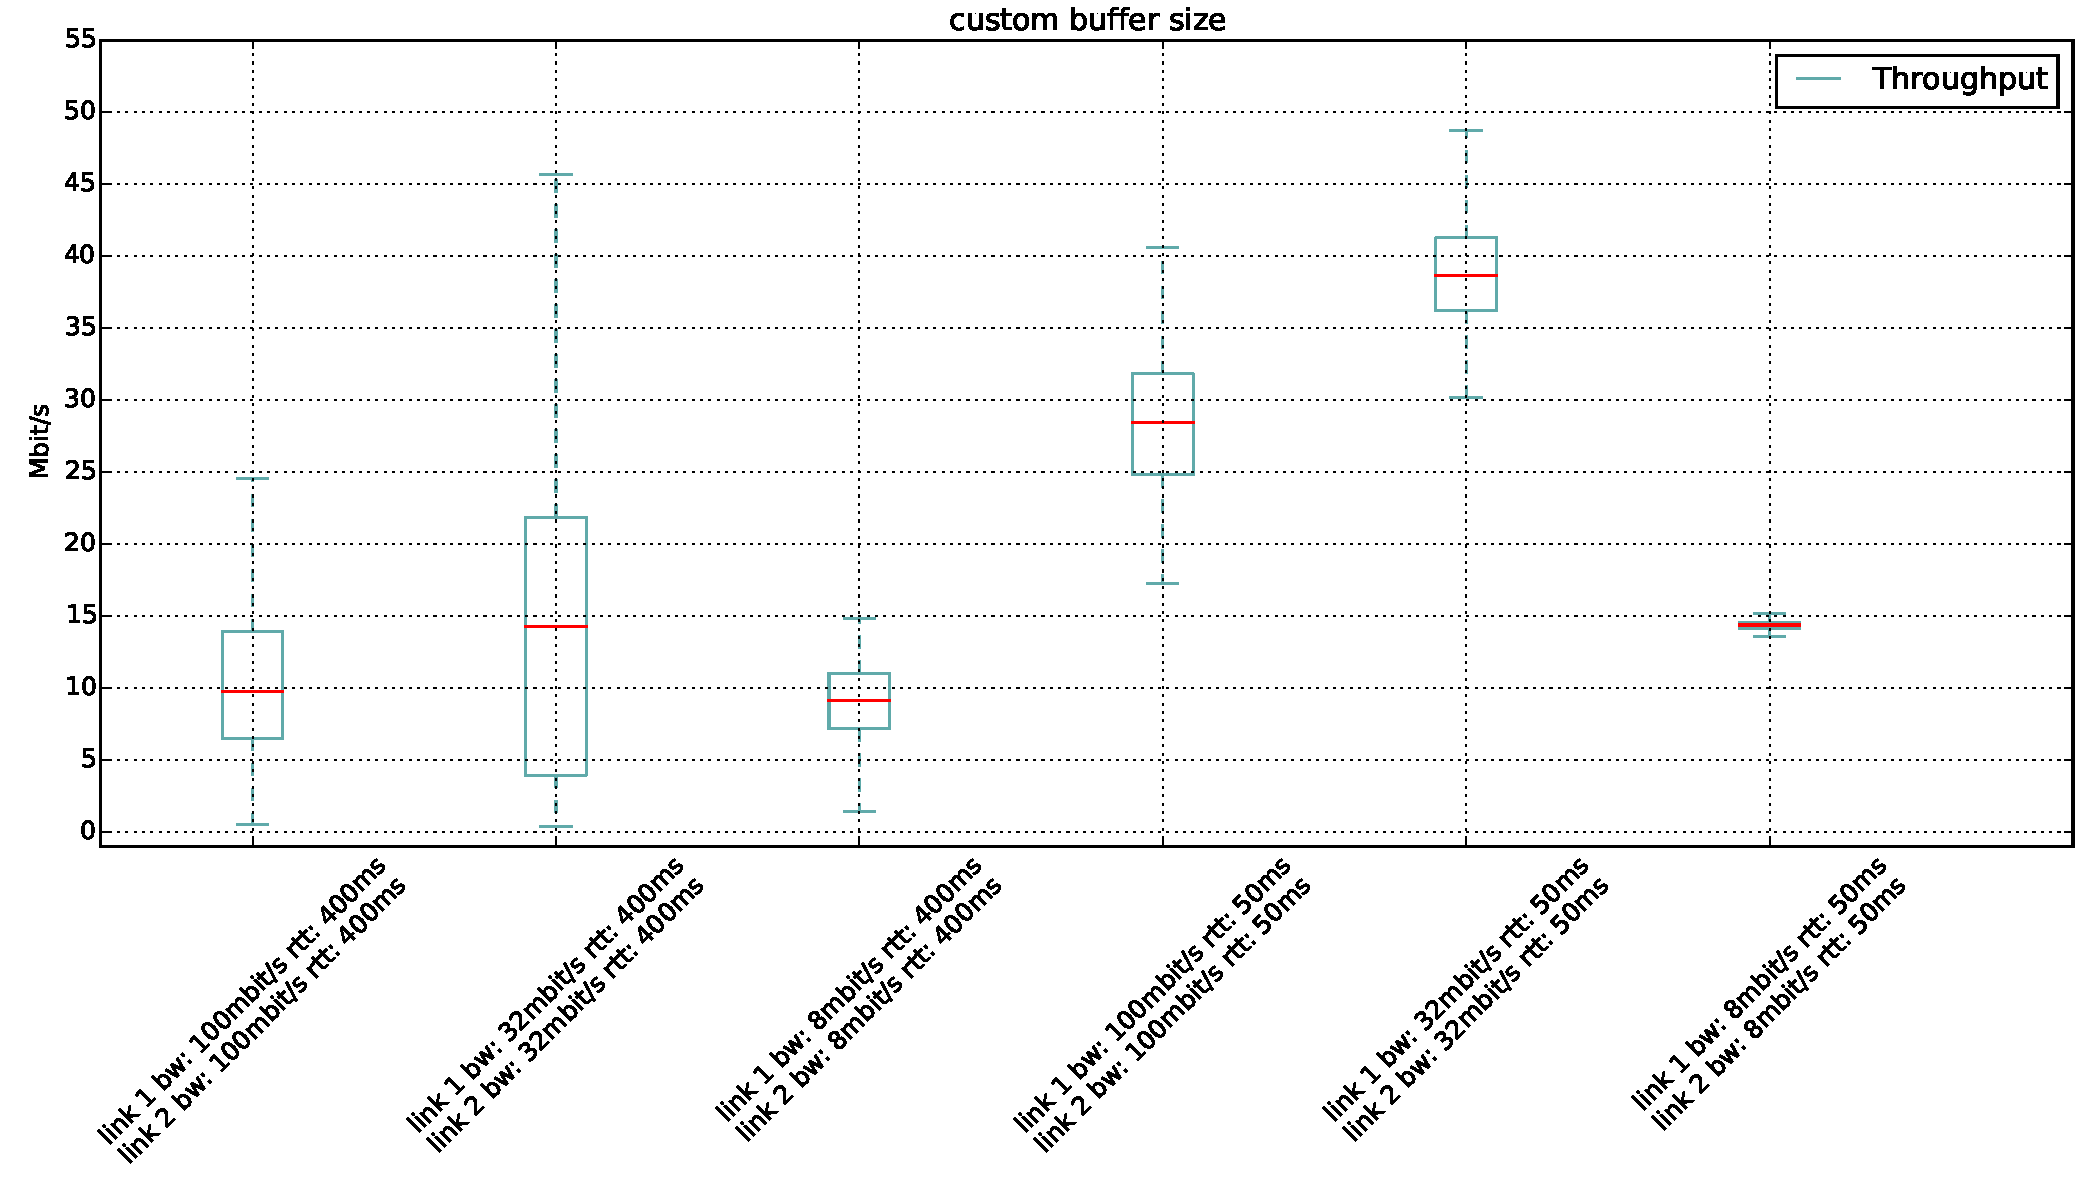
\includegraphics[width=1\textwidth]{../results/tcp_all_custom_buffer.pdf}
    \caption{TCP custom buffer size}
    \label{tcp_all_custom_buffer}
  \end{figure}

On figure \ref{tcp_all_custom_buffer} the same technique is applied for 32mbit/s and 100mbit/s.
It is interesting to see that it improves the throughput in every cases but it does not equal the results obtained with a 2ms RTT.
I tried many different buffer sizes but I was unable to match it.

There is also some unexpected results like the 100mbit/s links with a RTT of 50 only giving a throughput around 30 mbit/s. To but sure I have looked at the sender window but
it did not fill the receiver window, this was not the problem. Analysing the capture with MPTCPTrace I saw on the sequence graph some \"flat\" increase
suggesting that packet losses were happening. Using TCPTrace I looked at the encapsulated connection and indeed there was some packet losses which could be the reason for the
window not to increase.

Looking at the packet capture I determined that the higher RTT, the more retransmissions were occurring which implies a decrease in the throughput.

Another very interesting thing is that the retransmissions happens only in the encapsulated TCP connection. Because TCP over TCP is used, there is a upper layer
which is the OpenVPN packet supporting MPTCP and a lower layer, which is the traffic from the computer client with normal TCP encapsulated in the upper layer.

The retransmission could happen in both layers but here we observe that it only happens in the lower layer.
This is positive in the sense that it does not retransmit multiple times on the different layers, meaning that it does not have the TCP meltdown effect~\cite{tcpovertcp}.
This also tell us that the upper layer, the MPTCP connection is limited by the lower layer.

This is illustrated in figure \ref{upper_seq} and figure \ref{lower_seq}.
Figure \ref{upper_seq} shows the sequence graph generated with MPTCP on the upper layer TCP connection, it shows that the line is pretty flat between time 105 and 120.
Figure \ref{lower_seq} shows the sequence graph generated by TCPTrace on the lower layer TCP connection at time 105. On this figure a lot of SACK and some retransmissions are observable meaning
that there is packet losses at this time.

\begin{figure}[h!]
  \centering
  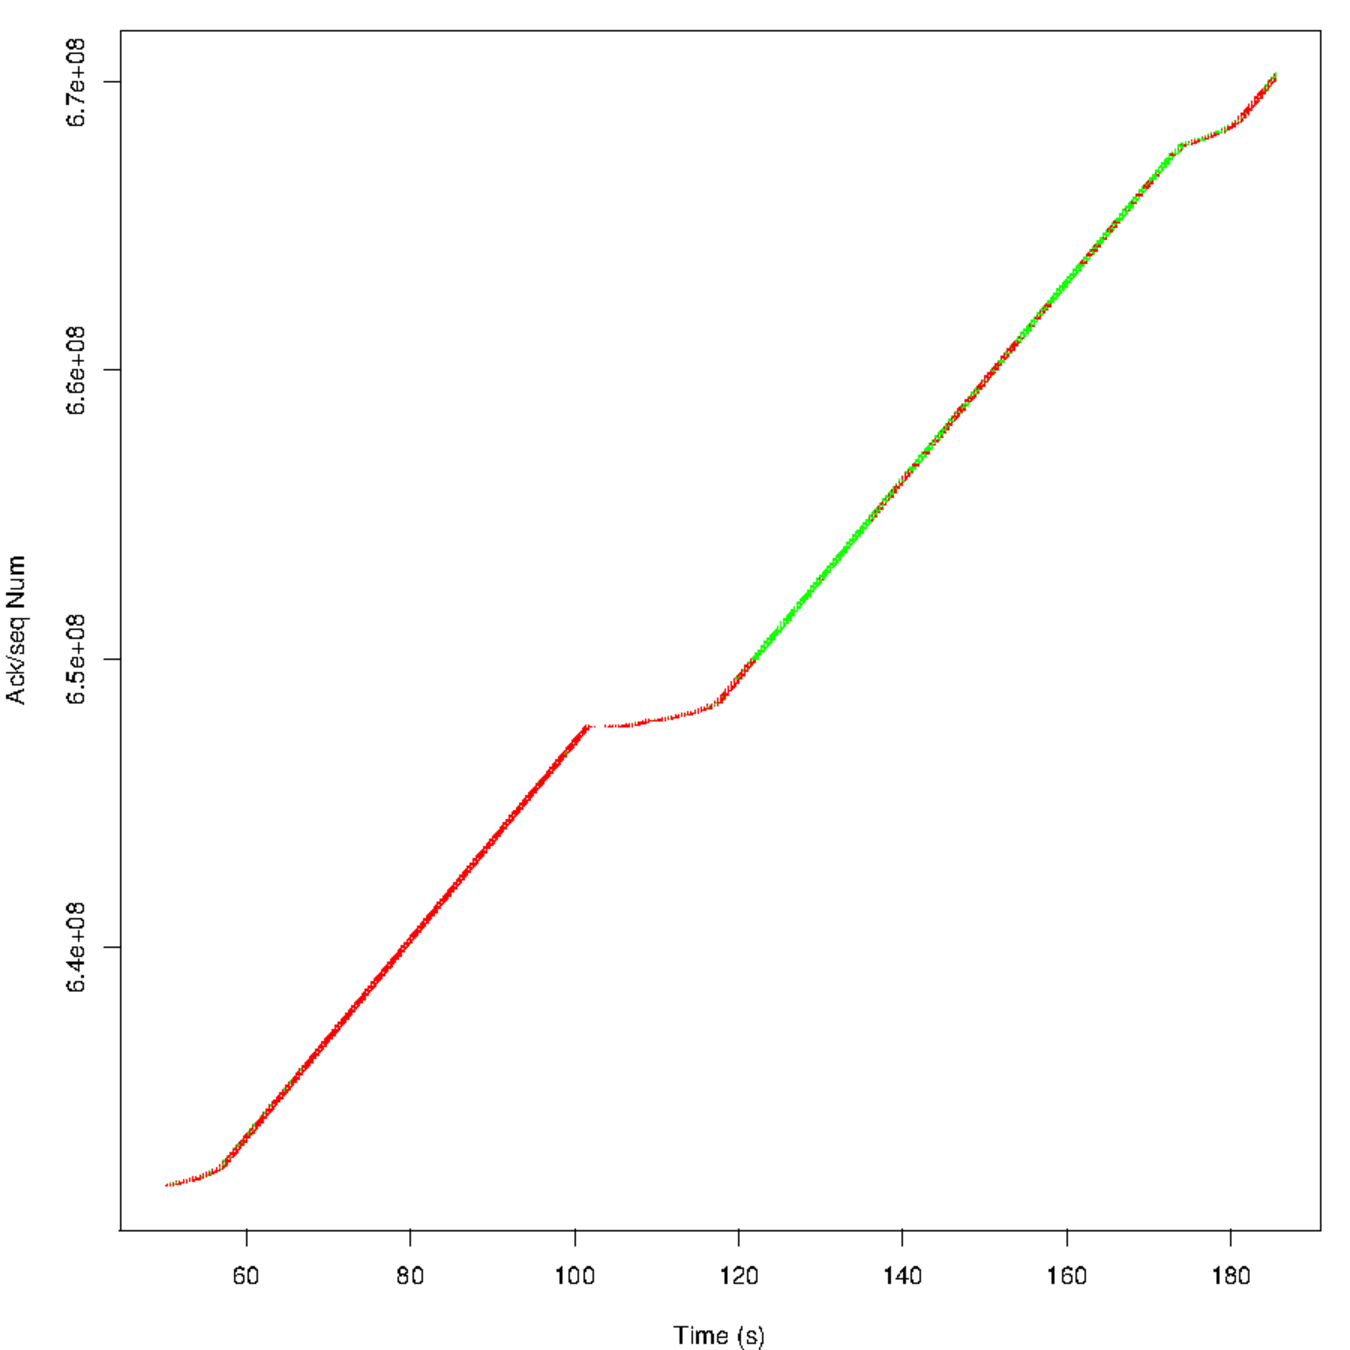
\includegraphics[width=10cm]{../results/upper_layer_seq.pdf}
  \caption{Sequence graph of the upper layer}
  \label{upper_seq}
\end{figure}

\begin{figure}[h!]
  \centering
  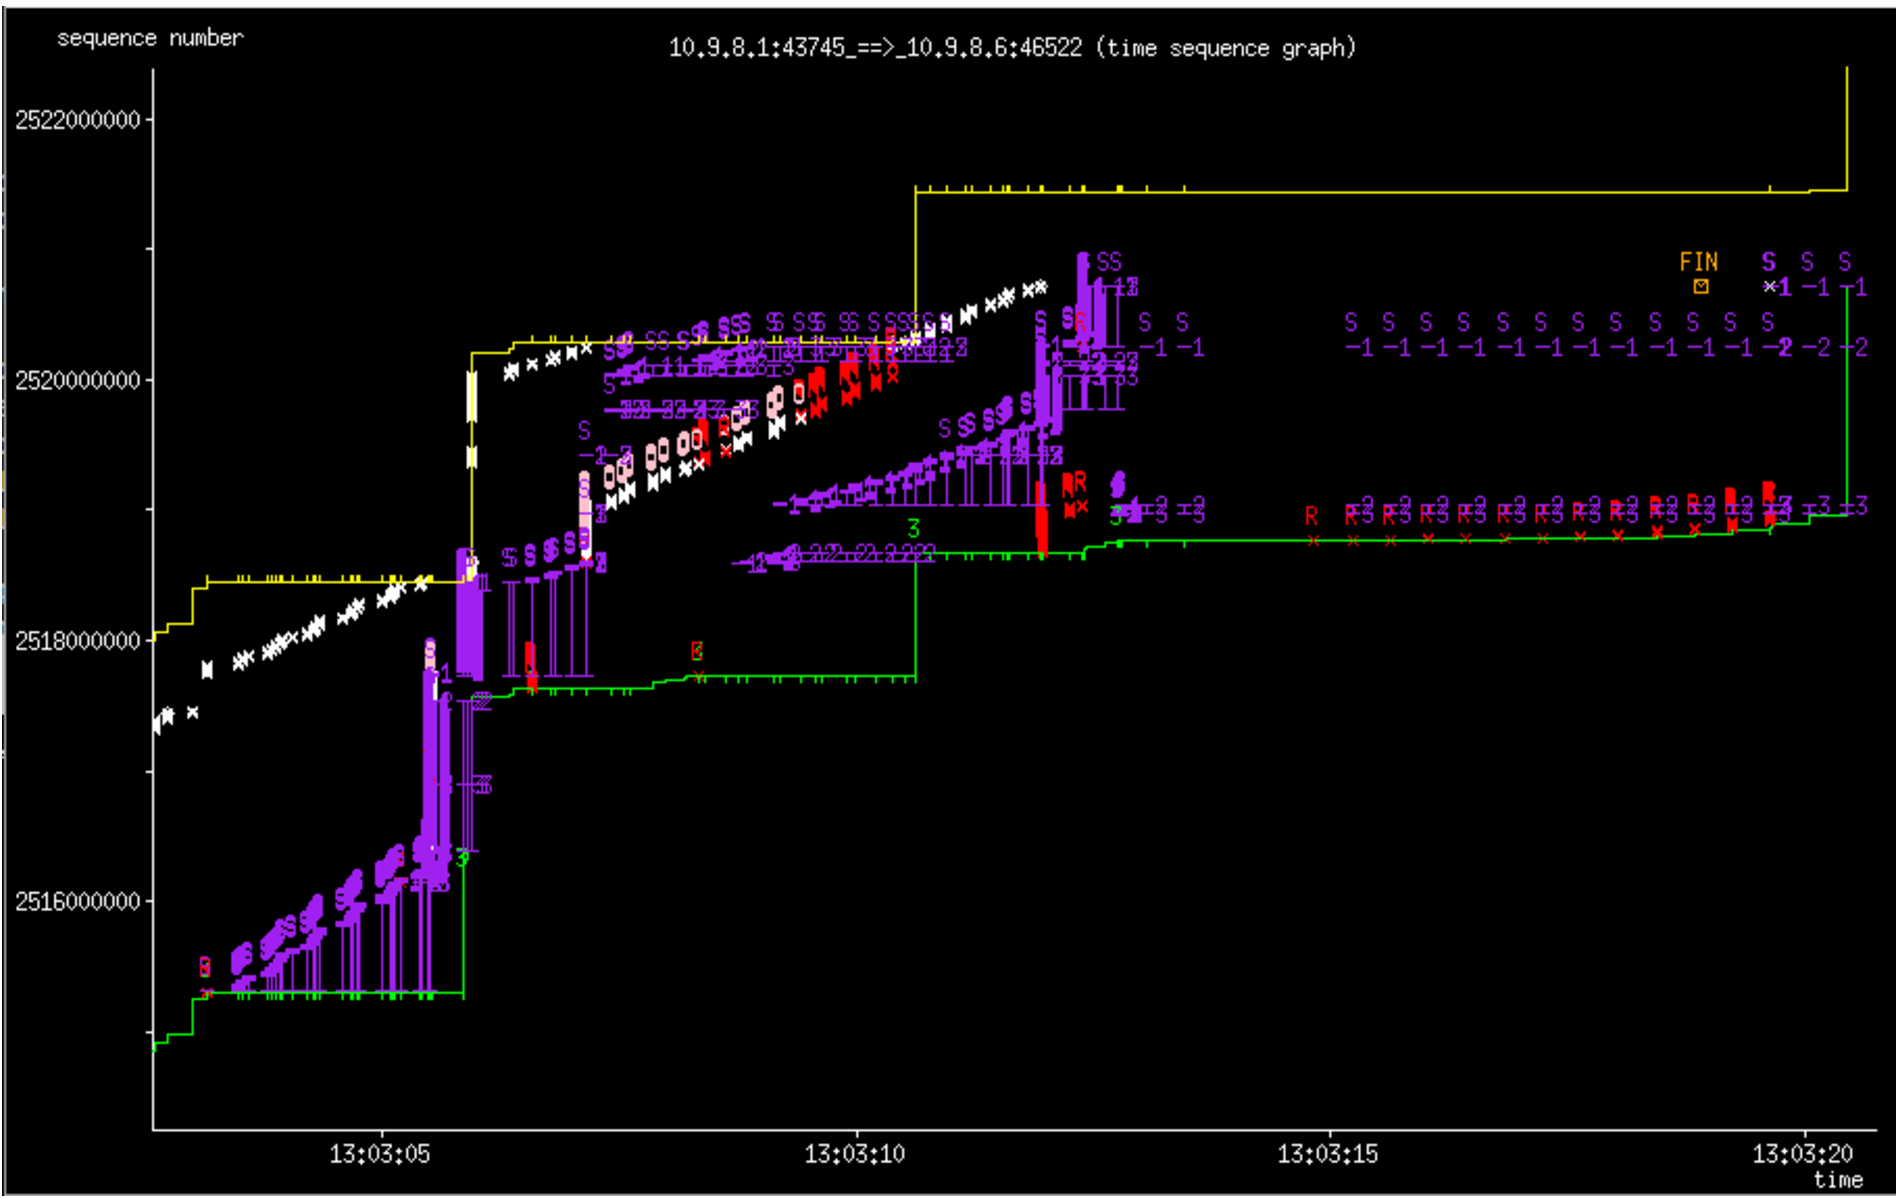
\includegraphics[width=10cm]{../results/lower_layer_seq.pdf}
  \caption{Sequence graph of the lower layer at time 105}
  \label{lower_seq}
\end{figure}

\section{Improving throughput by changing congestion control algorithm} \label{sec:improving_throughput_congestion_control}

In this test I will try switching between different congestion control algorithms, using cubic, lia, olia and wvegas, advised by Olivier Bonaventure and Benjamin Hesmans.

I first take the setup from the first test of section \ref{sec:bulk_data_transfer} to compare the results between the algorithms.

Figure \ref{all_congestion_algo_2rtt} shows that they all give similar results expect wvegas which use both subflow but keep the maximum throughput equivalent to the maximum throughput of only one link.

\begin{figure}[h!]
  \centering
  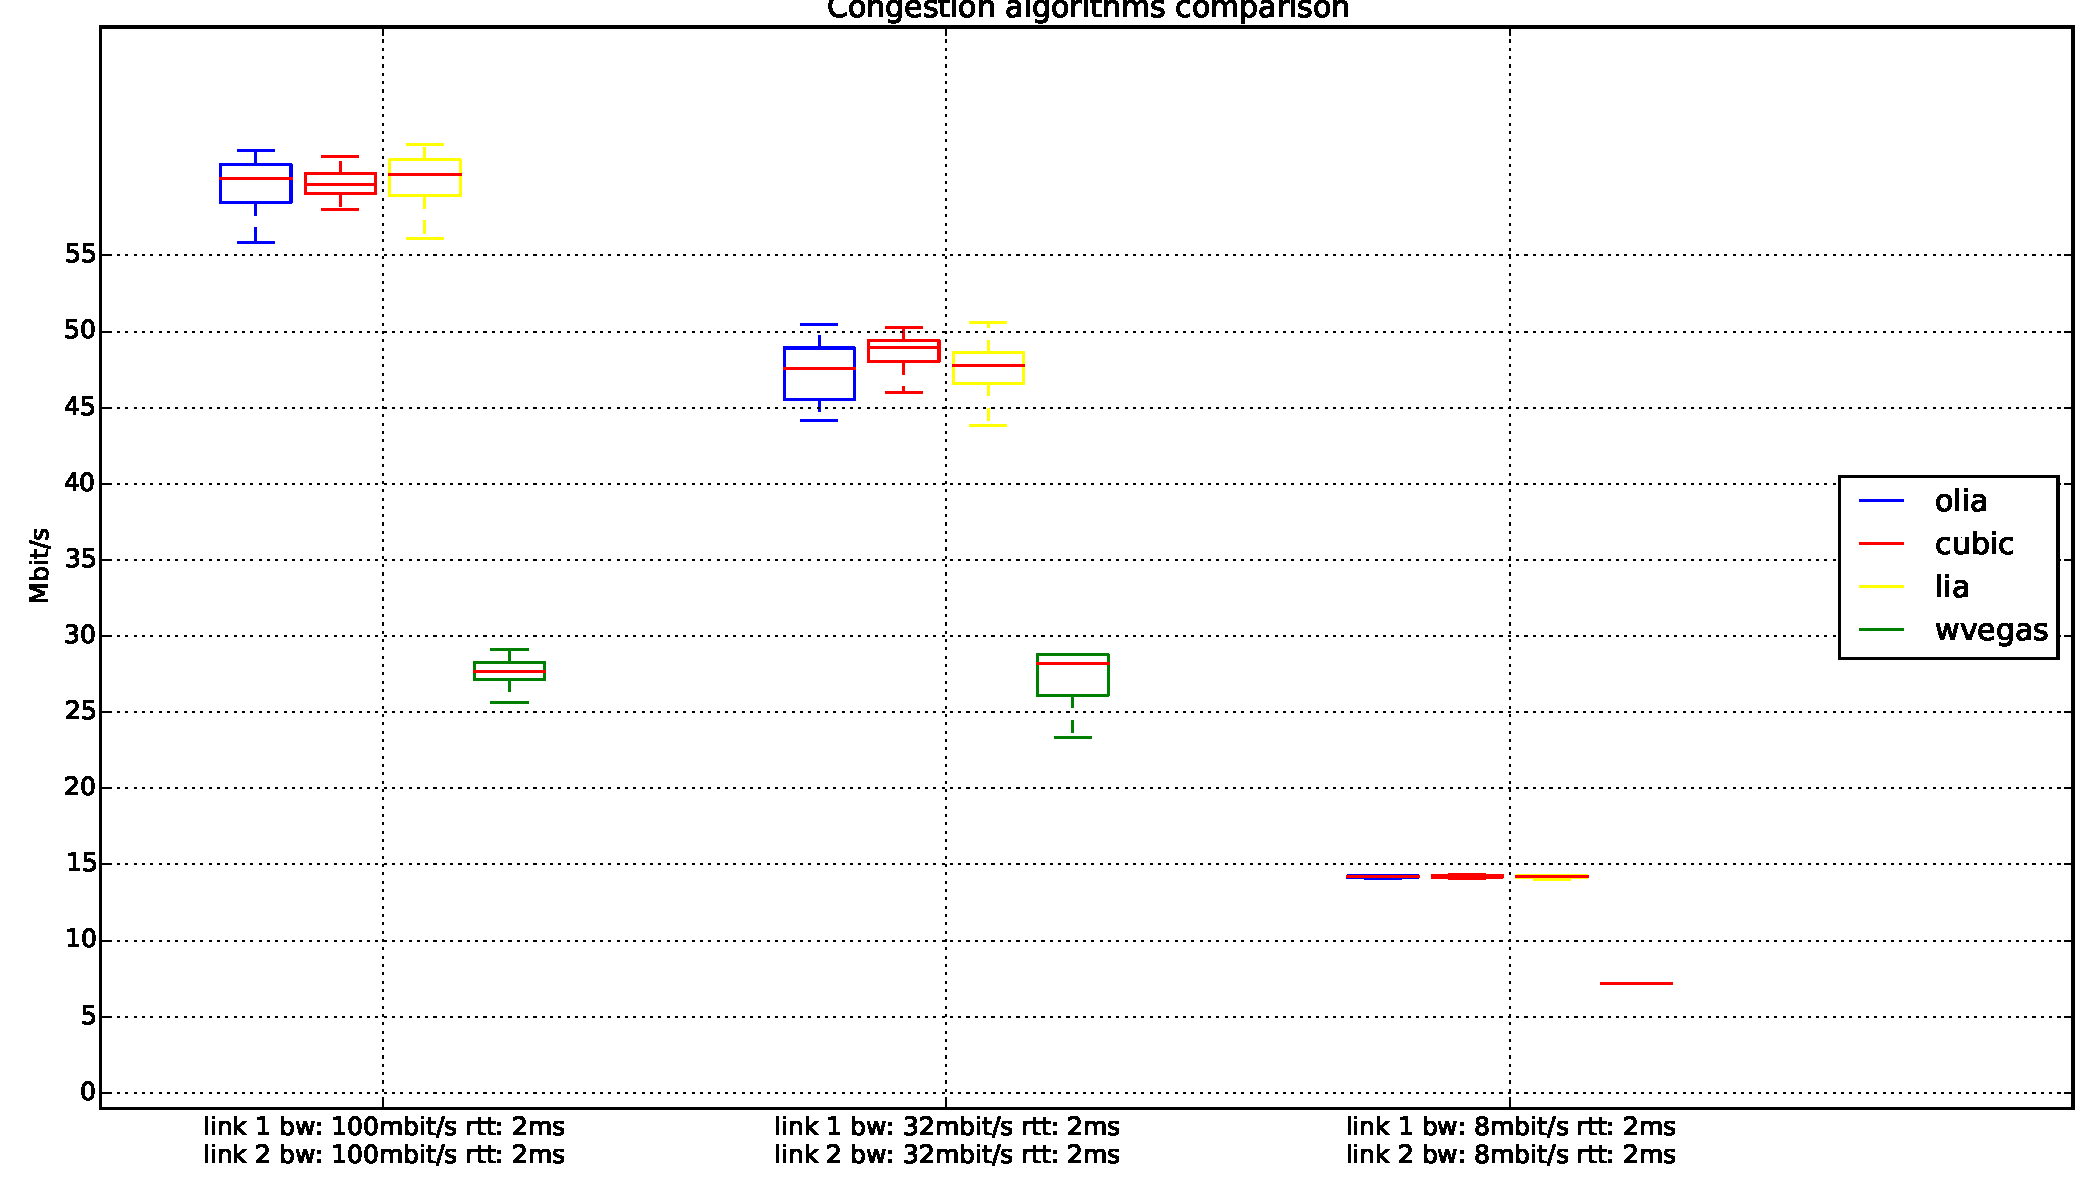
\includegraphics[width=1\textwidth]{../results/all_congestion_algo_2rrt.pdf}
  \caption{Congestion algorithms comparison}
  \label{all_congestion_algo_2rtt}
\end{figure}


Secondly I use setups from test \ref{sec:first_test} and \ref{sec:third_test} to determine wether the algorithms can make a better use of the two subflows when they have different bandwith and RTT.

Figure \ref{all_congestion_algo} show that for setup from section \ref{sec:first_test} the throughput is
almost the same accross all the algorithms except it is a bit lower for wvegas and olia. This is likely due to the fact that they are more fair to normal TCP compared to the others.

For setup from section \ref{sec:third_test}, the wvegas algorithm does not provide a very good throughput.

From paper \cite{cao2012delay}, the autors says that wvegas algorithm is not very efficient with High Delay Bandwith product link.
The cause is the slow start phase of wvegas being very short and switching to congestion avoidance very early.
I tried using a single link with a High delay and High bandwidth and it brought a very low throughput about 100kbit/s on a link with a bandwidth of 32mbit/s and a RTT 400.
Another thing wvegas seems to have a hard time with is link with different RTT, it will usually pick only the link having the lowest RTT and not use the link with the Highest RTT even
if it is not a huge RTT.

To determine what happened with wvegas, I analyzed the capture with MPTCPTrace and TCPTrace. MPTCPTrace showed that both subflow were used but the one with the lowest RTT was used more often.
Another interesting thing is that the TCP windows on the sender side was very small which would explain why we get this very low throughput (see figure \ref{sender_windows_size})

\begin{figure}[h!]
  \centering
  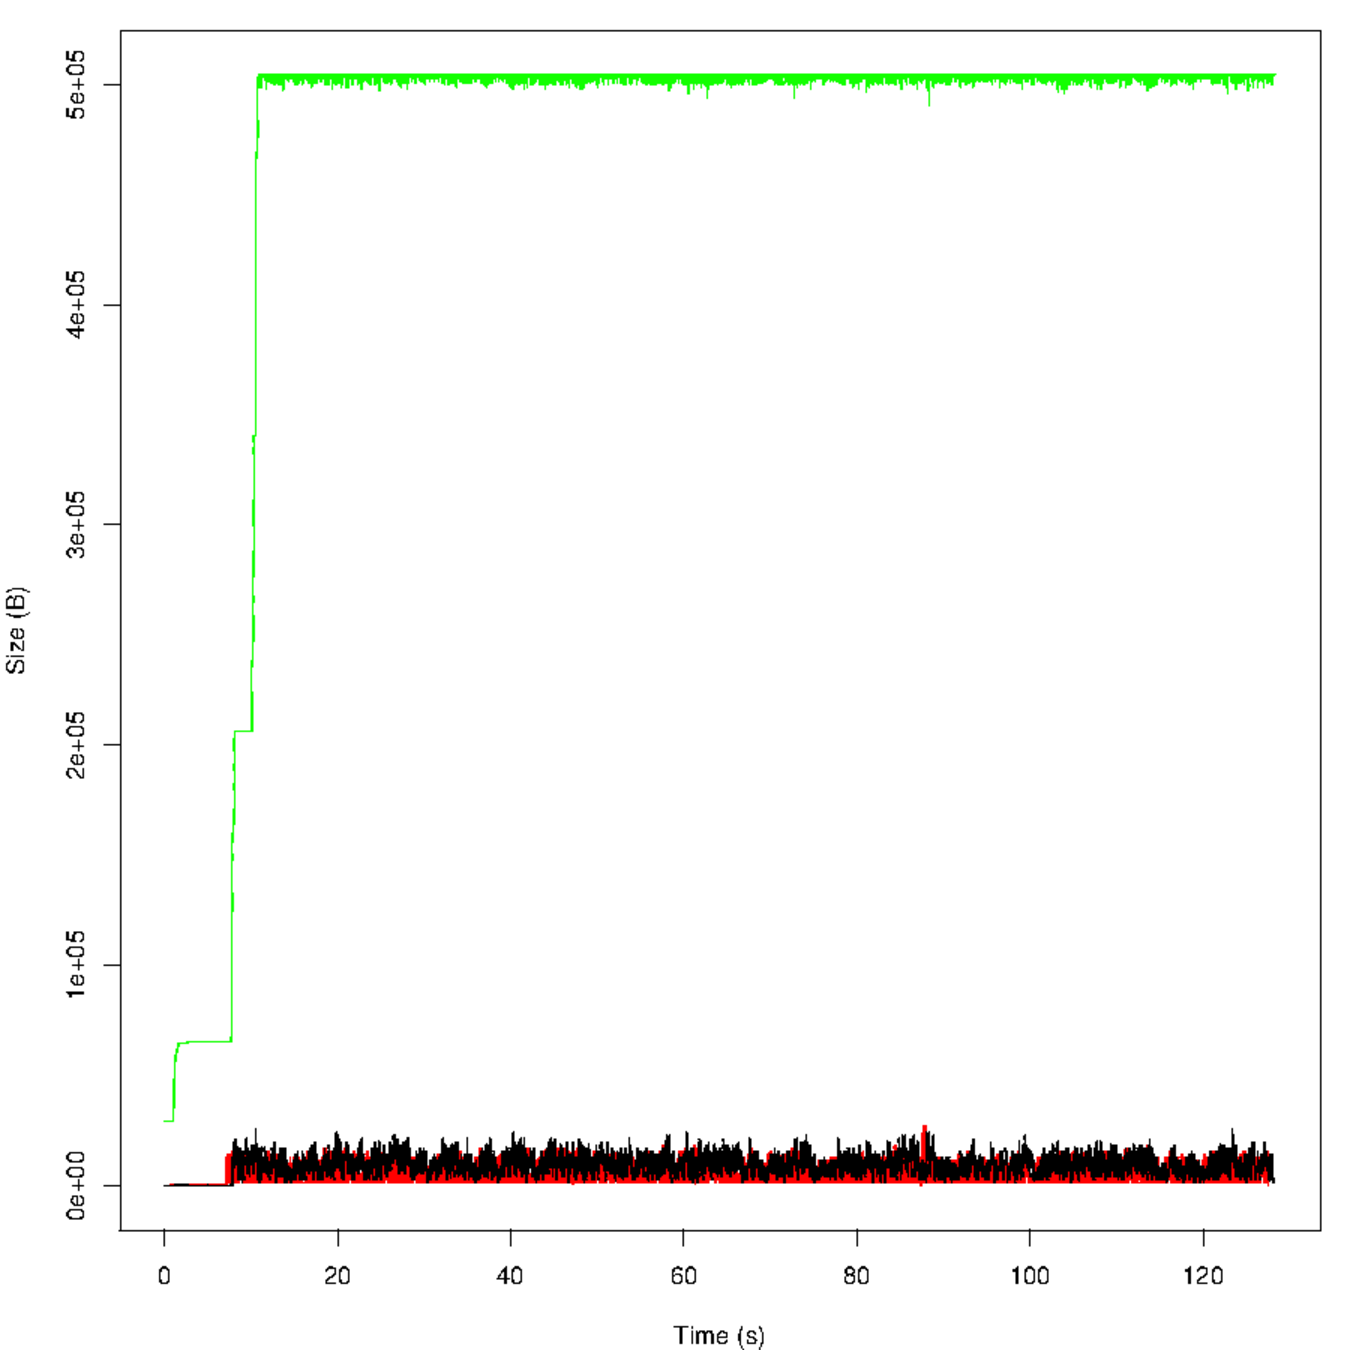
\includegraphics[width=8cm]{../results/window_wvegas_small.pdf}
  \caption{Sender windows size with wVegas}
  \label{sender_windows_size}
\end{figure}

\begin{figure}[h!]
  \centering
  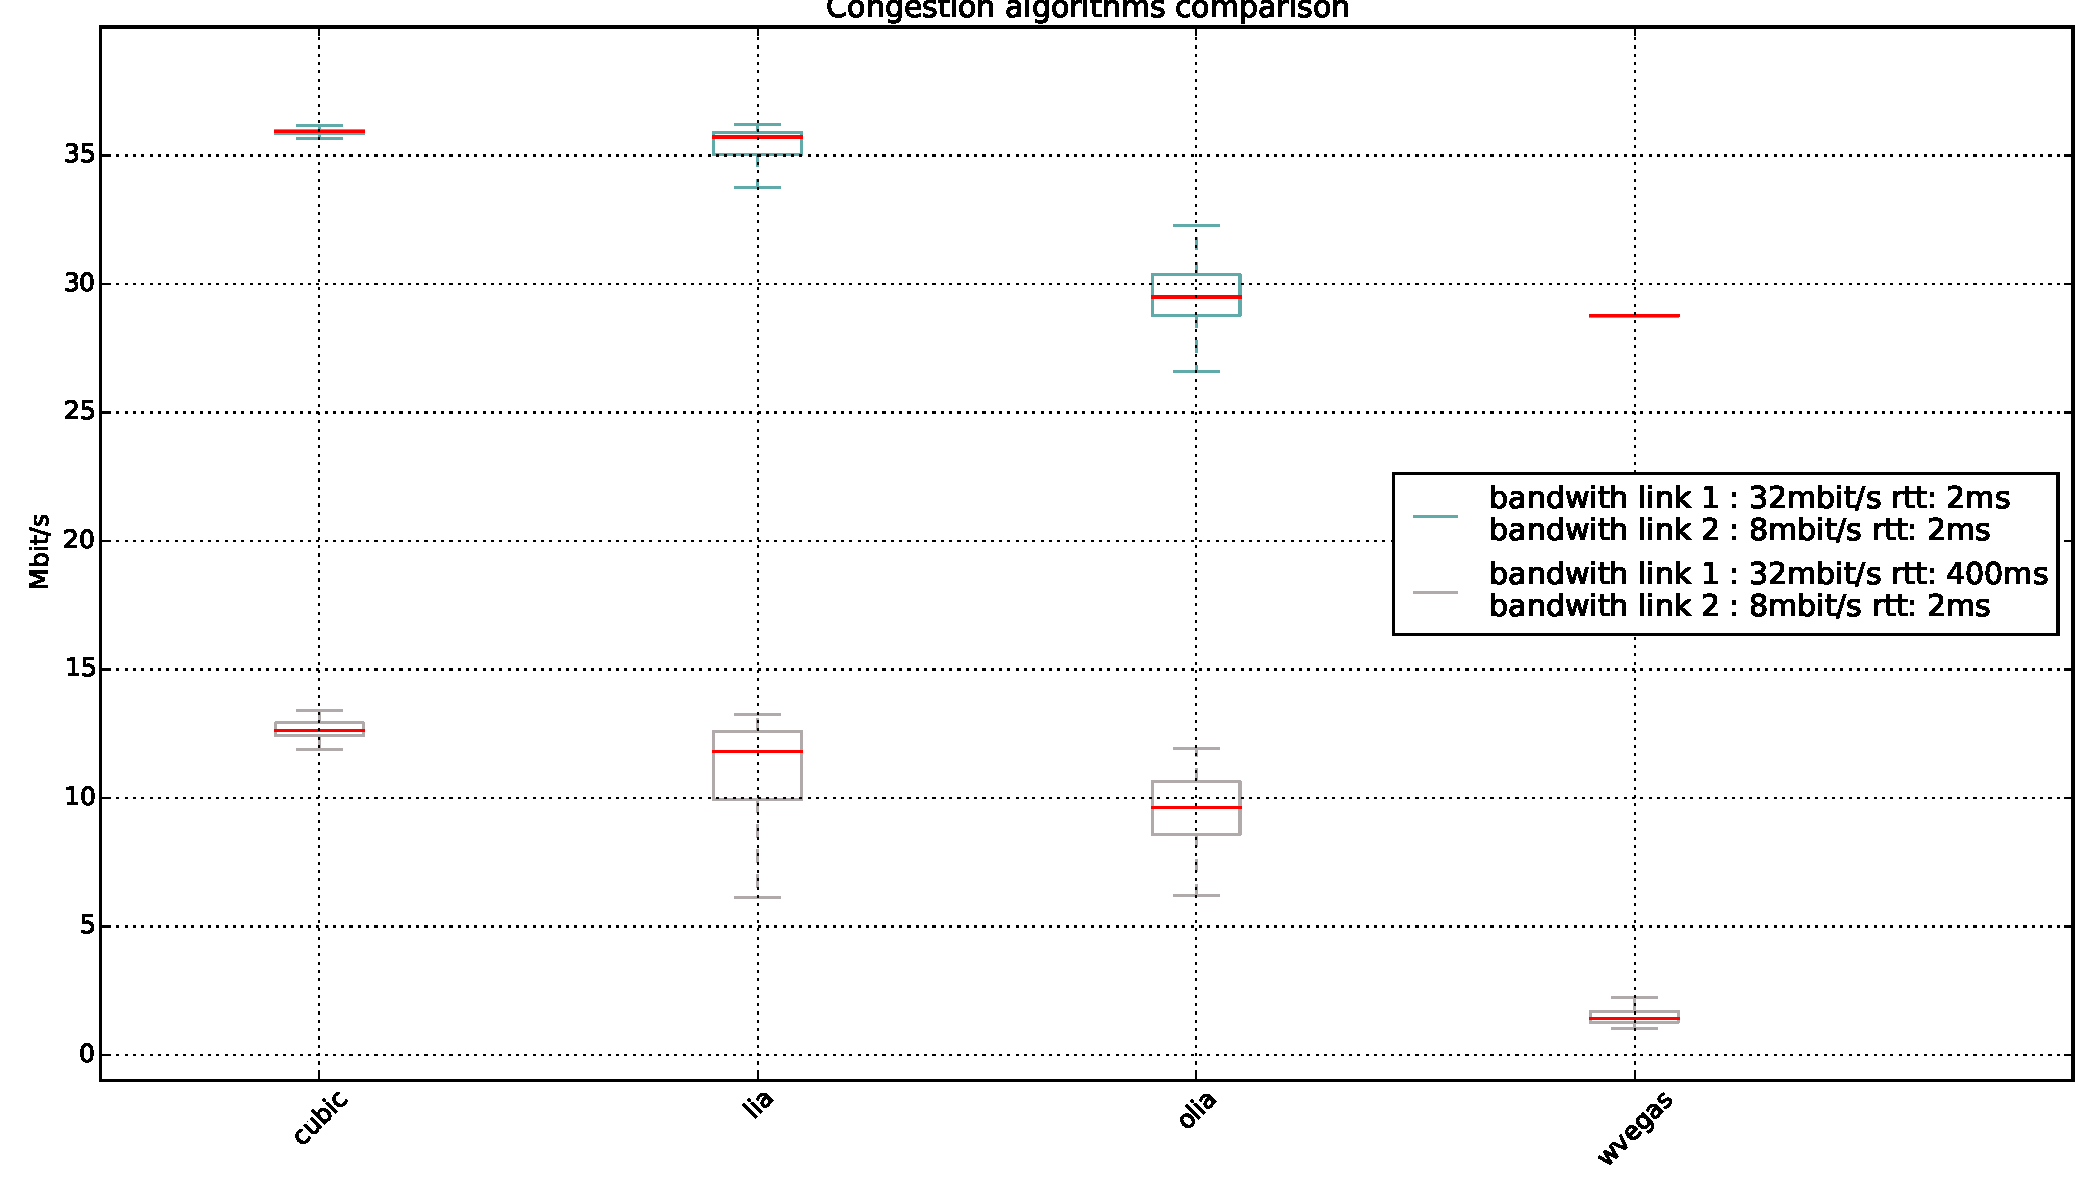
\includegraphics[width=1\textwidth]{../results/all_congestion_algo.pdf}
  \caption{Congestion algorithms comparison}
  \label{all_congestion_algo}
\end{figure}

\newpage

\section{Improving throughput by changing mptcp scheduler} \label{sec:improving_throughput_scheduler}


In test from section \ref{sec:third_test}, we saw that the MPTCP scheduler choose the subflow with the lowest RTT and from time to time use the subflow with the high RTT.
In this section I try to force MPTCP to use the High RTT subflow.

In this purpose I will change the MPTCP scheduler to Roundrobin and look at the effect on the overall throughput.
Roundrobin scheduler does not select subflow based on the RTT, it uses each subflow one after the other
(see section \ref{sec:mptcp_exp} for more information). The expectation is thus that the link with a high RTT will be used and the throughput will increase.

The RoundRobin will use $1$ as the \textit{num\_segments} parameter, number of consecutive segments that should be sent on one subflow and the parameter \textit{cwnd\_limited} will be set to \textit{true}
, the default value. The scheduler tries to fill the congestion window on all subflows.

The throughput with roundrobin is around 14mbit/s. Figure \ref{roundrobin} shows how the traffic was split across the two subflows. 

\begin{figure}[h!]
  \centering
  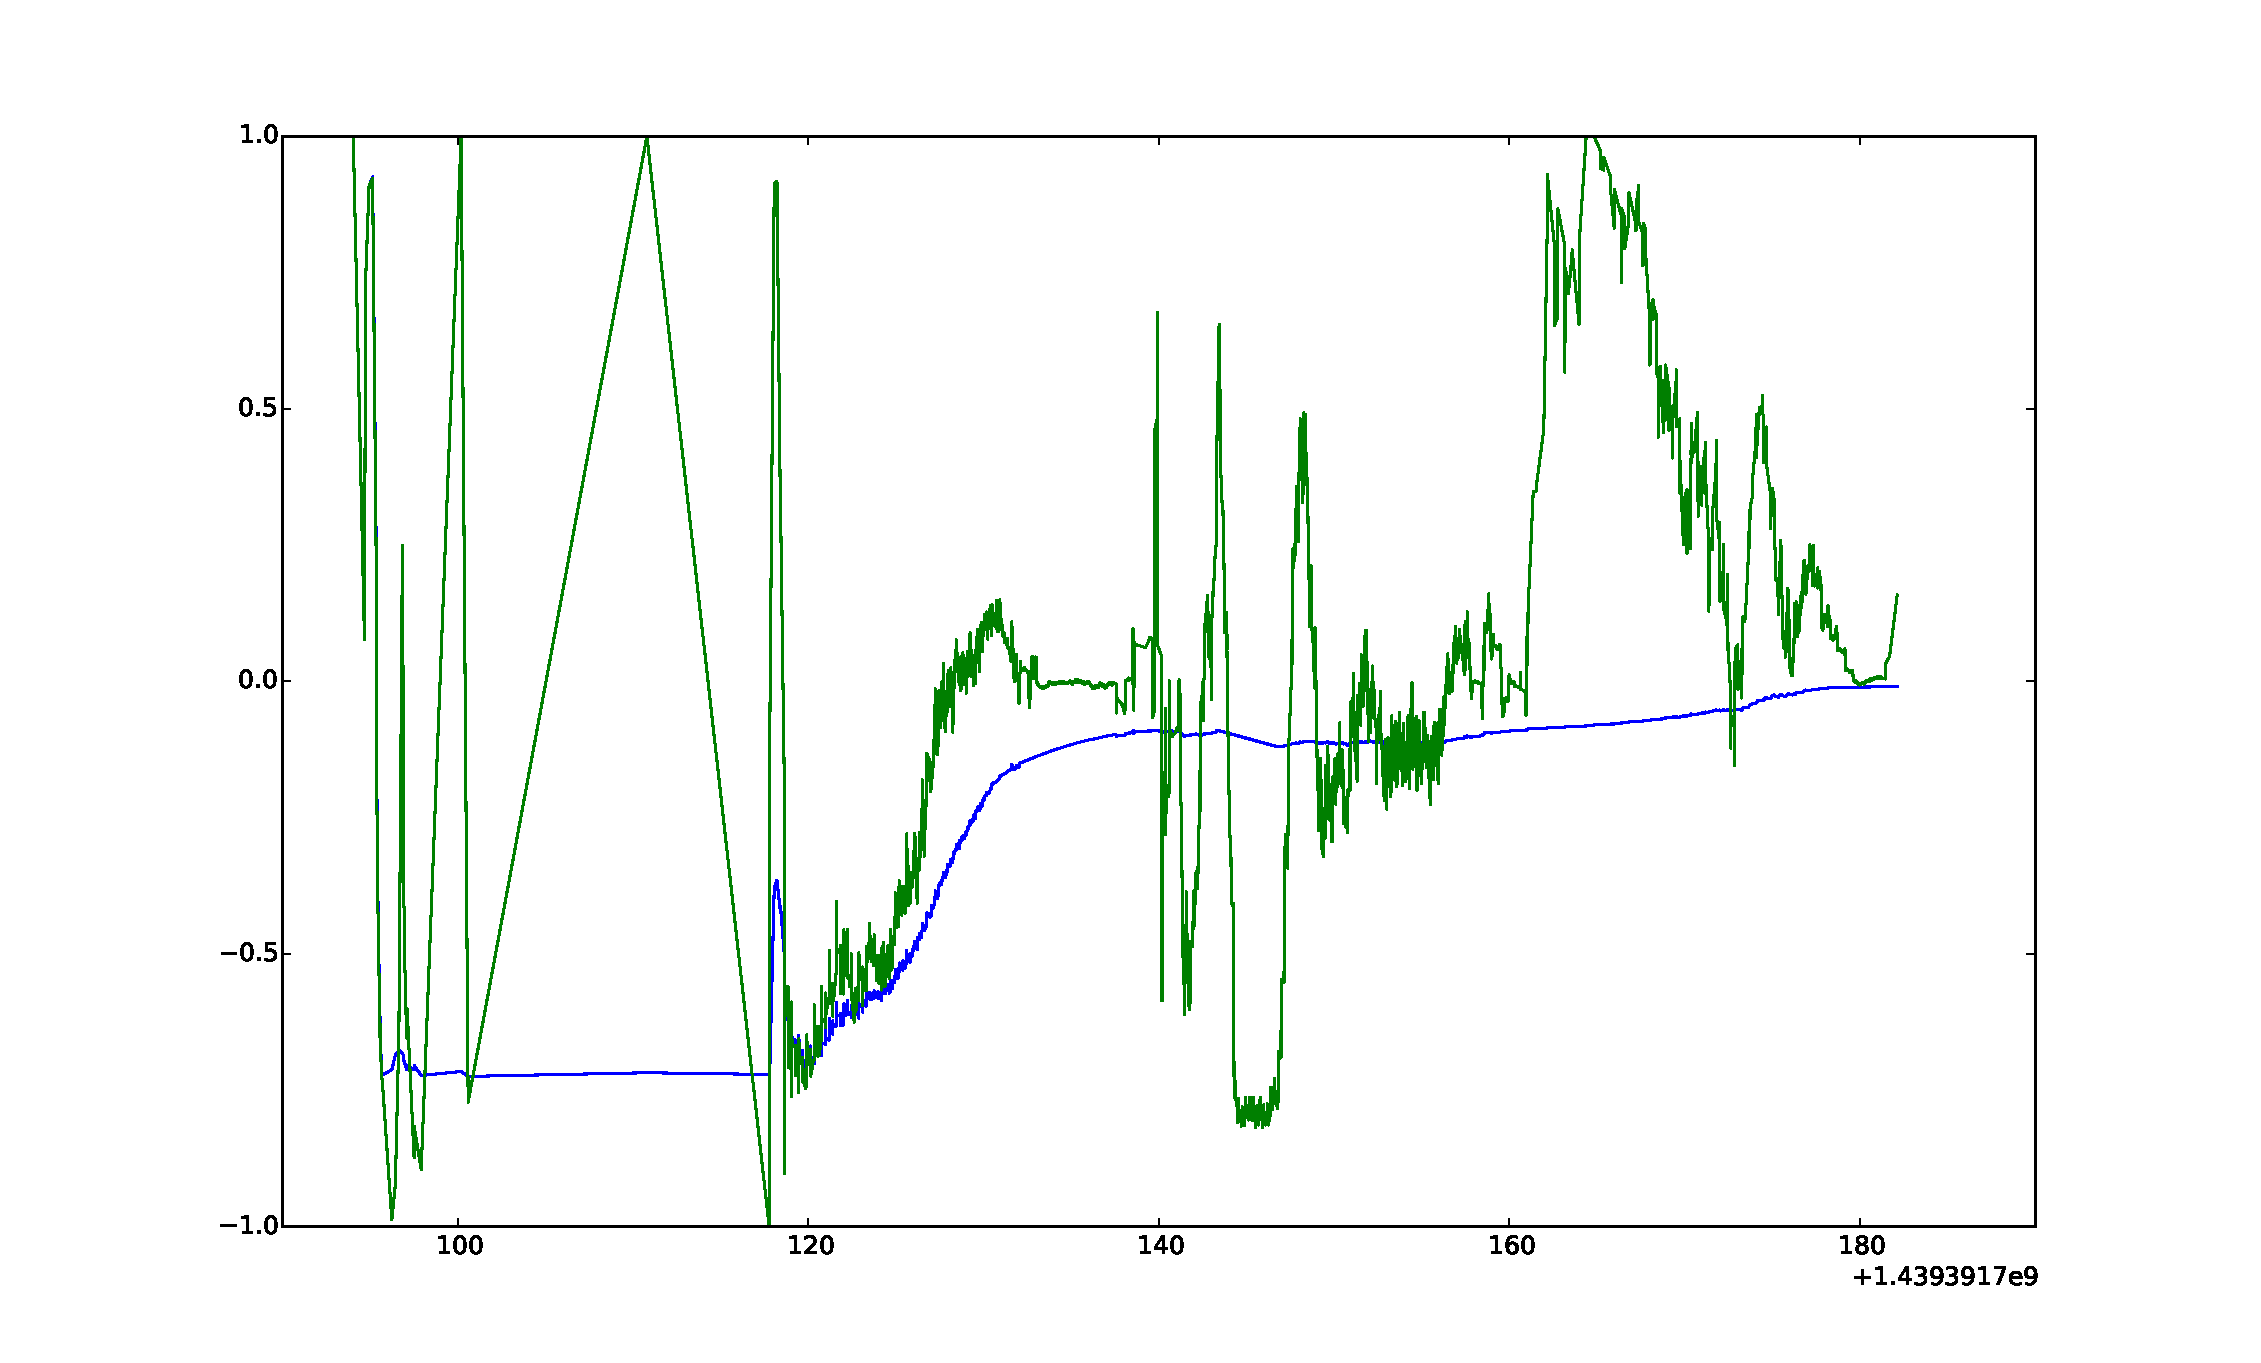
\includegraphics[width=1\textwidth]{../results/roundrobin.pdf}
  \caption{Roundrobin scheduler}
  \label{roundrobin}
\end{figure}


 \chapter{Tools}
  \section{Measurement tools}

  Here are the main tools used to gather and validate test data.

  \begin{itemize}
    \item Netperf and flent (netperf-wrapper) to measure the throughput
    \item Netperf and apache benchmark (AB) to measure request/response performance
    \item MPstat to check the CPU usage of the router and server
    \item Wireshark and TCPdump to capture packets
    \item MPTCTrace and TCPTrace to analyse captures
  \end{itemize}

  \subsection{netperf \autocite{netperf}}
  Netperf is a tool measuring network performance, compatible with TCP and UDP protocol. It has a client
  and a server. The server is netserver and listen to any client request and the client is used to iniate network test with the server.

  When you execute Netperf, the first thing that will happen is the establishment of a control connection to the remote system. This connection will be used to pass test configuration information and results to and from the remote system. Regardless of the type of test being run, the control connection will be a TCP connection using BSD sockets.

  Once the control connection is up and the configuration information has been passed, a separate connection will be opened for the measurement itself using the APIs and protocols appropriate for the test. The test will be performed, and the results will be displayed.
  Netperf places no traffic on the control connection while a test is in progress

  \subsection{flent (netperf-wrapper) \autocite{flent}}

  Netperf-wrapper, freshly called flent is a Python wrapper to run multiple simultaneous netperf/iperf/ping instances and aggregate the results. Tests are written in config files,
  test can be run several time using iterated tests. The results are saved into a JSON format to be processed later and multiple format can be choosen.

  It can also generate graphics like plotbox and cdf into different formats with the help of matplotlib. A batchfile can be writtent to automate test execution,
  This feature is very powerfull and I used it to perform multiple tests and adapt the bandwidth limit / delay on links.

  \subsection{mpstat}

  I used mpstat to check the CPU usage on the router. I wanted to identify the bootleneck which was limiting the bandwitdh
  and indeed it was using 100\% of the CPU when transmitting data throw the VPN.

  \subsection{Wireshark and TCPdump}

  TCPdump have been use to sniff packets that will later be analyse with MPTCPTrace and TCPTrace.

  Wireshark have been used make sure that the MPTCP protocol is in used during the tests,
  looking at MPTCP options like MP\_CAPABLE option, ADD\_ADDR option and MP\_JOIN.

  \subsection{MPTCPTrace \autocite{Hesmans:2014:TMT:2619239.2631453}}

  I used MPTCPTrace to analyse pcap captured by tcpdump on the server side and get more information about the MPTCP connection.
  I have used many of the graph produced by mptcptrace :

  \begin{itemize}
    \item The sequence graph to get an idea on how the traffic was distributed accross the different subflows and see if packets losses were happening
    \item The goodput graph to see how many goodput we could get and cross verify with the one from netperf.
    \item The flight and flight per flow graph to see the size of the TCP window
  \end{itemize}

  \subsection{TCPTrace \autocite{tcptrace}}

  To analyse the captured packets in more detail, I also used tcptrace. It was very helpfull to look at the sequence number graph of each subflow and
  see the packet lost on capture from the tun interface.


 \chapter{Conclusion}
 

  In conclusion, results of the tests show that providing a robust and fast internet connection to compagnies and individuals using MPTCP coupled with OpenVPN is something possible.

  The setup is minimal and not too expensive. The elements needed are two or more internet connections, a router running a MPTCP compatible kernel for the OpenVPN client and
  a server running a MPTCP compatible kernel for the OpenVPN server having a high bandwith.

  The basic configuration is simple but can be more complicated if the goal is to achieve good performances and try to maximize the speed of the internet connection.

  In term of performance, the hardware need to be powerfull enough otherwise the throughput will be limited by OpenVPN and its intensive
  use of the CPU to encapsulate and decapsulate packets. Here with the TP-LINK N900 router the maximum throughput it could reach was 57mbit/s before the CPU was saturated, with
  nowdays internet connection going up to 100mbit/s, this limit is not very high.

  In this paper we saw that using OpenVPN with MPTCP on links having low bandwith delay product gives good performance.
  However using links with high bandwith delay product decrease the performances.
  In some cases the use of MPTCP is not even worth it, UDP as the OpenVPN protocol would be a better choice in term of performances if we ommit the fact that it is less robust against failure.

  I have investigated and tried to solve the problem concerning the high bandwith delay product links with some level of success by adjusting the
  TCP windows size on both OpenVPN end side and trying different congestion algorithms.
  The performances were increased in every cases but depending on the configuration it was more or less significant.

  This being said, it will require internet connections to have a low RTT between the OpenVPN client and the OpenVPN server to get an acceptable user experience.
  Normal VDSL or ADSL connections should be adequate but mobile internet connection (3G) or sattelite internet connection will not be suitable for this kind of setup.

  Finally all the tests in this paper were done in a closed lab environnement. An interesting thing to do would be to try that in the real world environnement over the internet, to determine
  if additional problems than the ones represented in these experimental tests are encountered, potentially making the use of MPTCP coupled with OpenVPN not a viable solution.
  Another interesting thing would be to try using a different technology than OpenVPN and test if it would give better performances.


 \printbibliography

 \appendix
  \chapter{Annexes}
  Everything can be found in a git repository at this address : \url{https://github.com/alokhan/memoire}


\end{document}
